%% Time-stamp: <2019-02-01 09:10:32 (marc)>
\documentclass[xcolor=dvipsnames,compress, mathserif]{beamer}

\newcommand\hmmax{0}
\newcommand\bmmax{0}

\usepackage{../includes/MarkMathCmds}

\newcommand{\hackspace}{\hspace{4.2mm}}
\newcommand{\showstudent}[1]{}





% talk/author information
\newcommand{\authorname}{Mark van der Wilk}
\newcommand{\authoremail}{m.vdwilk@imperial.ac.uk}
\newcommand{\authoraffiliation}{
 Department of Computing\\Imperial
  College London}
\newcommand{\slidesettitle}{\imperialBlue{Logistic Regression \& \\ Laplace Approximation}}
\newcommand{\authortwitter}{markvanderwilk}
\newcommand{\footertitle}{Logistic Regression \& Laplace Approximation}
\newcommand{\location}{Imperial College London}
\newcommand{\talkDate}{{February 20, 2023}}


\date{\imperialGray{\talkDate}}




% load defaults
\selectcolormodel{rgb}
\usepackage{ifxetex,ifluatex}
\newif\ifxetexorluatex
\ifxetex
  \xetexorluatextrue
\else
  \ifluatex
    \xetexorluatextrue
  \else
    \xetexorluatexfalse
  \fi
\fi

\usepackage{textpos}
%\usepackage{arabtex}
\usepackage{tikz}
\usetikzlibrary{decorations.markings}
\usetikzlibrary{arrows}
\usetikzlibrary{shapes}
\usetikzlibrary{plotmarks}
\usetikzlibrary{mindmap,trees,backgrounds}

\tikzstyle{every picture}+=[remember picture]

%\usepackage{movie15}
% \usepackage{pdfpages}
%\usepackage{xmpmulti}

\usepackage{anyfontsize}
\usepackage{wrapfig}
\usepackage{animate}
\usepackage{multirow}
\usepackage{multimedia}
\usepackage{xmpmulti}
%\usepackage[latin9]{inputenc}
\usepackage[english]{babel}
\usepackage{scalefnt}
\usepackage{verbatim}
\usepackage{url}
% \usepackage{pgf,pgfarrows,pgfnodes}
\usepackage{textpos}
\usepackage[tight,ugly]{units}
\usepackage{url}
\usepackage{bbm}
\usepackage[english]{babel}
\usepackage{fancyhdr}
\usepackage{bm} % correct bold symbols, like \bm
\usepackage{amsmath}
\usepackage{amsfonts}
\usepackage{amssymb}
\usepackage{mathrsfs}
\usepackage{mathtools}
\usepackage{color}
\usepackage{cancel}
\usepackage{algorithm}
\usepackage{algpseudocode}
\usepackage{mathrsfs}
\usepackage{listings}
\usepackage{graphicx} % for pdf, bitmapped graphics files
\usepackage{mathtools}
\usepackage{units}
\usepackage{subfig}
\usepackage{enumerate}
\usepackage{natbib}
\usepackage{dsfont}


\ifxetexorluatex
\usepackage{fontspec}
\setmainfont[Scale=0.8]{OpenDyslexic-Regular}
\else
\usefonttheme{professionalfonts}
\fi

\renewcommand{\vec}[1]{{\boldsymbol{{#1}}}} % vector
\newcommand{\mat}[1]{{\boldsymbol{{#1}}}} % matrix
% \newcommand{\KL}[2]{\mathrm{KL}(#1\|#2)} % KL divergence
\newcommand{\R}[0]{\mathds{R}} % real numbers
\newcommand{\Z}[0]{\mathds{Z}} % integers
\newcommand{\tr}[0]{\text{tr}} % trace
% \newcommand{\inv}{^{-1}}
% \DeclareMathOperator*{\diag}{diag}
\newcommand{\E}{\mathds{E}} % expectation
\newcommand{\var}{\mathds{V}}
\newcommand{\gauss}[2]{\mathcal{N}\big(#1,\,#2\big)}
\newcommand{\gaussx}[3]{\mathcal{N}\big(#1\,|\,#2,\,#3\big)}
\newcommand{\gaussBig}[2]{\mathcal{N}\left(#1,\,#2\right)}
\newcommand{\gaussxBig}[3]{\mathcal{N}\left(#1\,\left|\,#2,\,#3\right.\right)}
\newcommand{\Ber}[0]{\mathrm{Ber}} % Bernoulli distribution
\DeclareMathOperator{\cov}{Cov}
\ifxetexorluatex
\renewcommand{\T}[0]{^\top}
\renewcommand{\d}[0]{\text{d}} % derivative
\else
\newcommand{\T}[0]{^\top}
\renewcommand{\d}[0]{\text{d}} % derivative
\fi
% calculus
\newcommand{\pdiff}[1]{\frac{\partial}{\partial #1}}
\newcommand{\pdiffF}[2]{\frac{\partial #1}{\partial #2}}
\newcommand{\diffF}[2]{\frac{{\d}#1}{{\d}#2}}
\newcommand{\diffFII}[2]{\frac{{\d}^2 #1}{{\d}#2^2}}
\newcommand{\diff}[1]{\frac{{\d}}{{\d}#1}}
\newcommand{\diffII}[1]{\frac{{\d}^2}{{\d}#1^2}}
\newcommand{\class}[0]{\mathcal{C}}

\newcommand{\idx}[1]{^{(#1)}}
% \newcommand{\norm}[1]{\left\|#1\right\|}
\newcommand{\proj}[1]{\tilde{#1}}
\newcommand{\pcacoord}{z}
\newcommand{\pcacoordnew}{\zeta}
\newcommand{\latent}{z}
% \newcommand{\given}{\,|\,}
\newcommand{\genset}[1]{\mathrm{span}[#1]} % generating set
\newcommand{\set}[1]{\mathcal{#1}} % set
\newcommand{\fixgmfont}[1]{\scalebox{0.8}{#1}}



\usepackage{pifont}% http://ctan.org/pkg/pifont
\newcommand{\cmark}{{\color{green!40!black}\ding{51}}}%
\newcommand{\xmark}{{\color{red}\ding{55}}}%
\newcommand{\green}[1]{{\bf{\textcolor{green}{#1}}}}
\newcommand{\red}[1]{{\bf{\textcolor{red}{#1}}}}

\newcommand<>\red[1]{{\color#2[rgb]{1,0,0}#1}}
\newcommand<>\blue[1]{{\color#2[rgb]{0,0,1}#1}}
\newcommand<>\yellow[1]{{\color#2{camyellow}#1}}
\newcommand<>\green[1]{{\color#2[rgb]{0,0.6,0.0}#1}}
\newcommand<>\violet[1]{{\color#2[rgb]{0.6,0,0.6}#1}}
\newcommand<>\orange[1]{{\color#2[rgb]{1,0.5,0}#1}}
\newcommand<>\black[1]{{\color#2[rgb]{0,0,0}#1}}
\newcommand<>\steel[1]{{\color#2[rgb]{0,0,0.8}#1}}
\newcommand<>\darkblue[1]{{\color#2[rgb]{0,0,0.6}#1}}
\newcommand<>\lightblue[1]{{\color#2[rgb]{0.4,0.4,0.7}#1}}
\newcommand<>\gray[1]{{\color#2[rgb]{0.4,0.4,0.4}#1}}
\newcommand<>\greenish[1]{{\color#2[rgb]{0.45, 0.66, 0.45}#1}}
\newcommand<>\redish[1]{{\color#2[rgb]{0.7843    0.3706    0.3706}#1}}
\definecolor{redishTIKZ}{rgb}{0.7843, 0.3706, 0.3706}
\definecolor{imperialBlue}{rgb}{0.058, 0.219, 0.418}
\definecolor{aimsbrown}{rgb}{0.539, 0.117, 0.015}
% \definecolor{imperialGray}{rgb}{0.414, 0.488, 0.671 }
\definecolor{imperialGray}{RGB}{109,153, 204}
\definecolor{aimslightbrown}{RGB}{138,88,84}
\newcommand<>\imperialBlue[1]{{\color#2[rgb]{0.058, 0.219, 0.418}#1}}
\newcommand<>\aimsbrown[1]{{\color#2[rgb]{0.539, 0.117, 0.015}#1}}
%\newcommand<>\imperialGray[1]{{\color#2[rgb]{0.414, 0.488, 0.671}#1}}
\newcommand<>\imperialGray[1]{{\color#2[RGB]{109,153, 204}#1}}
\newcommand<>\aimslightbrown[1]{{\color#2[RGB]{138,88,84}#1}}
\newcommand<>\lightgray[1]{{\color#2[rgb]{0.8,0.8,0.8}#1}}
%\newcommand<>\highlightcolor[1]{{\color#2[rgb]{0,0,1}#1}}
\newcommand{\highlight}[1]{{\bf\steel{#1}}}
%\newcommand{\newblock}[0]{}

%\newcommand{\arrow}[0]{\includegraphics[height=5pt]{./figures/arrow}\hspace{3pt}}

\renewcommand{\emph}[1]{\textbf{\steel{{#1}}}}

\renewcommand{\alert}[1]{{\bf\red{{#1}}}}

\newcommand{\arrow}{
\begin{tikzpicture}
\draw [black!40!green, fill=black!40!green] (0,-0.12) -- (0,0.12) --
(0.15,0);
\draw [black!40!green, fill=black!40!green] (0.15,-0.12) -- (0.15,0.12) --
(0.3,0); 
\end{tikzpicture}
}

\geometry{left=0.45cm,top=0cm,right=0.45cm}


\newcommand{\logoimagepath}{./figures/imperial}
\newcommand{\highlightcolor}{blue!80!black}
%\newcommand{\headbarcolor}{imperialBlue}
\newcommand{\headbarcolor}{imperialBlue}
\institute{}

\newcommand{\coursetitle}{}

\newcommand{\slidesetsubtitle}{}
\newcommand{\slidesetnumber}{01}
\usefonttheme{professionalfonts}


\usetikzlibrary{decorations.fractals}
% tikzlibrary.code.tex
%
% Copyright 2010-2011 by Laura Dietz
% Copyright 2012 by Jaakko Luttinen
%
% The MIT License
%
% See LICENSE file for more details.

% Load other libraries
\usetikzlibrary{shapes}
\usetikzlibrary{fit}
\usetikzlibrary{chains}
\usetikzlibrary{arrows}

% Latent node
\tikzstyle{latent} = [circle,fill=white,draw=black,inner sep=1pt,
minimum size=20pt, font=\fontsize{10}{10}\selectfont, node distance=1]
% Observed node
\tikzstyle{obs} = [latent,fill=gray!25]
% Constant node
\tikzstyle{const} = [rectangle, inner sep=0pt, node distance=1]
% Factor node
\tikzstyle{factor} = [rectangle, fill=black,minimum size=5pt, inner
sep=0pt, node distance=0.4]
% Deterministic node
\tikzstyle{det} = [latent, diamond]

% Plate node
\tikzstyle{plate} = [draw, rectangle, rounded corners, fit=#1]
% Invisible wrapper node
\tikzstyle{wrap} = [inner sep=0pt, fit=#1]
% Gate
\tikzstyle{gate} = [draw, rectangle, dashed, fit=#1]

% Caption node
\tikzstyle{caption} = [font=\footnotesize, node distance=0] %
\tikzstyle{plate caption} = [caption, node distance=0, inner sep=0pt,
below left=5pt and 0pt of #1.south east] %
\tikzstyle{factor caption} = [caption] %
\tikzstyle{every label} += [caption] %

%\pgfdeclarelayer{b}
%\pgfdeclarelayer{f}
%\pgfsetlayers{b,main,f}

% \factoredge [options] {inputs} {factors} {outputs}
\newcommand{\factoredge}[4][]{ %
  % Connect all nodes #2 to all nodes #4 via all factors #3.
  \foreach \f in {#3} { %
    \foreach \x in {#2} { %
      \path (\x) edge[-,#1] (\f) ; %
      %\draw[-,#1] (\x) edge[-] (\f) ; %
    } ;
    \foreach \y in {#4} { %
      \path (\f) edge[->, >={triangle 45}, #1] (\y) ; %
      %\draw[->,#1] (\f) -- (\y) ; %
    } ;
  } ;
}

% \edge [options] {inputs} {outputs}
\newcommand{\edge}[3][]{ %
  % Connect all nodes #2 to all nodes #3.
  \foreach \x in {#2} { %
    \foreach \y in {#3} { %
      \path (\x) edge [->, >={triangle 45}, #1] (\y) ;%
      %\draw[->,#1] (\x) -- (\y) ;%
    } ;
  } ;
}

% \factor [options] {name} {caption} {inputs} {outputs}
\newcommand{\factor}[5][]{ %
  % Draw the factor node. Use alias to allow empty names.
  \node[factor, label={[name=#2-caption]#3}, name=#2, #1,
  alias=#2-alias] {} ; %
  % Connect all inputs to outputs via this factor
  \factoredge {#4} {#2-alias} {#5} ; %
}

% \plate [options] {name} {fitlist} {caption}
\newcommand{\plate}[4][]{ %
  \node[wrap=#3] (#2-wrap) {}; %
  \node[plate caption=#2-wrap] (#2-caption) {#4}; %
  \node[plate=(#2-wrap)(#2-caption), #1] (#2) {}; %
}

% \gate [options] {name} {fitlist} {inputs}
\newcommand{\gate}[4][]{ %
  \node[gate=#3, name=#2, #1, alias=#2-alias] {}; %
  \foreach \x in {#4} { %
    \draw [-*,thick] (\x) -- (#2-alias); %
  } ;%
}

% \vgate {name} {fitlist-left} {caption-left} {fitlist-right}
% {caption-right} {inputs}
\newcommand{\vgate}[6]{ %
  % Wrap the left and right parts
  \node[wrap=#2] (#1-left) {}; %
  \node[wrap=#4] (#1-right) {}; %
  % Draw the gate
  \node[gate=(#1-left)(#1-right)] (#1) {}; %
  % Add captions
  \node[caption, below left=of #1.north ] (#1-left-caption)
  {#3}; %
  \node[caption, below right=of #1.north ] (#1-right-caption)
  {#5}; %
  % Draw middle separation
  \draw [-, dashed] (#1.north) -- (#1.south); %
  % Draw inputs
  \foreach \x in {#6} { %
    \draw [-*,thick] (\x) -- (#1); %
  } ;%
}

% \hgate {name} {fitlist-top} {caption-top} {fitlist-bottom}
% {caption-bottom} {inputs}
\newcommand{\hgate}[6]{ %
  % Wrap the left and right parts
  \node[wrap=#2] (#1-top) {}; %
  \node[wrap=#4] (#1-bottom) {}; %
  % Draw the gate
  \node[gate=(#1-top)(#1-bottom)] (#1) {}; %
  % Add captions
  \node[caption, above right=of #1.west ] (#1-top-caption)
  {#3}; %
  \node[caption, below right=of #1.west ] (#1-bottom-caption)
  {#5}; %
  % Draw middle separation
  \draw [-, dashed] (#1.west) -- (#1.east); %
  % Draw inputs
  \foreach \x in {#6} { %
    \draw [-*,thick] (\x) -- (#1); %
  } ;%
}


% Copyright (C) 2016  Joseph Rabinoff

% ipe2tikz is free software; you can redistribute it and/or modify it under
% the terms of the GNU General Public License as published by the Free
% Software Foundation; either version 3 of the License, or (at your option)
% any later version.

% ipe2tikz is distributed in the hope that it will be useful, but WITHOUT ANY
% WARRANTY; without even the implied warranty of MERCHANTABILITY or FITNESS
% FOR A PARTICULAR PURPOSE.  See the GNU General Public License for more
% details.

% You should have received a copy of the GNU General Public License along with
% ipe2tikz; if not, you can find it at "http://www.gnu.org/copyleft/gpl.html",
% or write to the Free Software Foundation, Inc., 675 Mass Ave, Cambridge, MA
% 02139, USA.


% ipe compatibility TikZ styles

\usetikzlibrary{arrows.meta}

\makeatletter

% These should behave almost exactly like ipe arrows.  They disable correcting
% for the miter length and line width.  This is important for visual consistency
% with ipe, since ipe arrows get much larger when the line width is increased.
% They also use the line join and cap styles from the main path.  These are very
% simple arrows: there is no harpoon version, and the convex hull computation is
% sloppy.

\pgfdeclarearrow{
  name = ipe _linear,
  defaults = {
    length = +1bp,
    width  = +.666bp,
    line width = +0pt 1,
  },
  setup code = {
    % Control points
    \pgfarrowssetbackend{0pt}
    \pgfarrowssetvisualbackend{
      \pgfarrowlength\advance\pgf@x by-.5\pgfarrowlinewidth}
    \pgfarrowssetlineend{\pgfarrowlength}
    \ifpgfarrowreversed
      \pgfarrowssetlineend{\pgfarrowlength\advance\pgf@x by-.5\pgfarrowlinewidth}
    \fi
    \pgfarrowssettipend{\pgfarrowlength}
    % Convex hull
    \pgfarrowshullpoint{\pgfarrowlength}{0pt}
    \pgfarrowsupperhullpoint{0pt}{.5\pgfarrowwidth}
    % The following are needed in the code:
    \pgfarrowssavethe\pgfarrowlinewidth
    \pgfarrowssavethe\pgfarrowlength
    \pgfarrowssavethe\pgfarrowwidth
  },
  drawing code = {
    \pgfsetdash{}{+0pt}
    \ifdim\pgfarrowlinewidth=\pgflinewidth\else\pgfsetlinewidth{+\pgfarrowlinewidth}\fi
    \pgfpathmoveto{\pgfqpoint{0pt}{.5\pgfarrowwidth}}
    \pgfpathlineto{\pgfqpoint{\pgfarrowlength}{0pt}}
    \pgfpathlineto{\pgfqpoint{0pt}{-.5\pgfarrowwidth}}
    \pgfusepathqstroke
  },
  parameters = {
    \the\pgfarrowlinewidth,%
    \the\pgfarrowlength,%
    \the\pgfarrowwidth,%
  },
}


\pgfdeclarearrow{
  name = ipe _pointed,
  defaults = {
    length = +1bp,
    width  = +.666bp,
    inset  = +.2bp,
    line width = +0pt 1,
  },
  setup code = {
    % Control points
    \pgfarrowssetbackend{0pt}
    \pgfarrowssetvisualbackend{\pgfarrowinset}
    \pgfarrowssetlineend{\pgfarrowinset}
    \ifpgfarrowreversed
      \pgfarrowssetlineend{\pgfarrowlength}
    \fi
    \pgfarrowssettipend{\pgfarrowlength}
    % Convex hull
    \pgfarrowshullpoint{\pgfarrowlength}{0pt}
    \pgfarrowsupperhullpoint{0pt}{.5\pgfarrowwidth}
    \pgfarrowshullpoint{\pgfarrowinset}{0pt}
    % The following are needed in the code:
    \pgfarrowssavethe\pgfarrowinset
    \pgfarrowssavethe\pgfarrowlinewidth
    \pgfarrowssavethe\pgfarrowlength
    \pgfarrowssavethe\pgfarrowwidth
  },
  drawing code = {
    \pgfsetdash{}{+0pt}
    \ifdim\pgfarrowlinewidth=\pgflinewidth\else\pgfsetlinewidth{+\pgfarrowlinewidth}\fi
    \pgfpathmoveto{\pgfqpoint{\pgfarrowlength}{0pt}}
    \pgfpathlineto{\pgfqpoint{0pt}{.5\pgfarrowwidth}}
    \pgfpathlineto{\pgfqpoint{\pgfarrowinset}{0pt}}
    \pgfpathlineto{\pgfqpoint{0pt}{-.5\pgfarrowwidth}}
    \pgfpathclose
    \ifpgfarrowopen
      \pgfusepathqstroke
    \else
      \ifdim\pgfarrowlinewidth>0pt\pgfusepathqfillstroke\else\pgfusepathqfill\fi
    \fi
  },
  parameters = {
    \the\pgfarrowlinewidth,%
    \the\pgfarrowlength,%
    \the\pgfarrowwidth,%
    \the\pgfarrowinset,%
    \ifpgfarrowopen o\fi%
  },
}


% For correcting minipage width in stretched nodes
\newdimen\ipeminipagewidth
\def\ipestretchwidth#1{%
  \pgfmathsetlength{\ipeminipagewidth}{#1/\ipenodestretch}}

\tikzstyle{ipe import} = [
  % General ipe defaults
  x=1bp, y=1bp,
%
  % Nodes
  ipe node stretch/.store in=\ipenodestretch,
  ipe stretch normal/.style={ipe node stretch=1},
  ipe stretch normal,
  ipe node/.style={
    anchor=base west, inner sep=0, outer sep=0, scale=\ipenodestretch
  },
%
  % Use a special key for the mark scale, so that the default can be overriden.
  % (This doesn't happen with the scale= key; those accumulate.)
  ipe mark scale/.store in=\ipemarkscale,
%
  ipe mark tiny/.style={ipe mark scale=1.1},
  ipe mark small/.style={ipe mark scale=2},
  ipe mark normal/.style={ipe mark scale=3},
  ipe mark large/.style={ipe mark scale=5},
%
  ipe mark normal, % Set default
%
  ipe circle/.pic={
    \draw[line width=0.2*\ipemarkscale]
      (0,0) circle[radius=0.5*\ipemarkscale];
    \coordinate () at (0,0);
  },
  ipe disk/.pic={
    \fill (0,0) circle[radius=0.6*\ipemarkscale];
    \coordinate () at (0,0);
  },
  ipe fdisk/.pic={
    \filldraw[line width=0.2*\ipemarkscale]
      (0,0) circle[radius=0.5*\ipemarkscale];
    \coordinate () at (0,0);
  },
  ipe box/.pic={
    \draw[line width=0.2*\ipemarkscale, line join=miter]
      (-.5*\ipemarkscale,-.5*\ipemarkscale) rectangle
      ( .5*\ipemarkscale, .5*\ipemarkscale);
    \coordinate () at (0,0);
  },
  ipe square/.pic={
    \fill
      (-.6*\ipemarkscale,-.6*\ipemarkscale) rectangle
      ( .6*\ipemarkscale, .6*\ipemarkscale);
    \coordinate () at (0,0);
  },
  ipe fsquare/.pic={
    \filldraw[line width=0.2*\ipemarkscale, line join=miter]
      (-.5*\ipemarkscale,-.5*\ipemarkscale) rectangle
      ( .5*\ipemarkscale, .5*\ipemarkscale);
    \coordinate () at (0,0);
  },
  ipe cross/.pic={
    \draw[line width=0.2*\ipemarkscale, line cap=butt]
      (-.5*\ipemarkscale,-.5*\ipemarkscale) --
      ( .5*\ipemarkscale, .5*\ipemarkscale)
      (-.5*\ipemarkscale, .5*\ipemarkscale) --
      ( .5*\ipemarkscale,-.5*\ipemarkscale);
    \coordinate () at (0,0);
  },
%
  % Arrow sizes (for TikZ arrows)
  /pgf/arrow keys/.cd,
  ipe arrow normal/.style={scale=1},
  ipe arrow tiny/.style={scale=.4},
  ipe arrow small/.style={scale=.7},
  ipe arrow large/.style={scale=1.4},
  ipe arrow normal,
  /tikz/.cd,
%
  % Approximations to ipe arrows
  % Put in a style to allow to reset default scale when "ipe arrow normal" is
  % changed.  I think this is the only way, since all the parameters to arrows
  % are expanded when the tip is declared.
  ipe arrows/.style={
    ipe normal/.tip={
      ipe _pointed[length=1bp, width=.666bp, inset=0bp,
                   quick, ipe arrow normal]},
    ipe pointed/.tip={
      ipe _pointed[length=1bp, width=.666bp, inset=0.2bp,
                   quick, ipe arrow normal]},
    ipe linear/.tip={
      ipe _linear[length = 1bp, width=.666bp,
                  ipe arrow normal, quick]},
    ipe fnormal/.tip={ipe normal[fill=white]},
    ipe fpointed/.tip={ipe pointed[fill=white]},
    ipe double/.tip={ipe normal[] ipe normal},
    ipe fdouble/.tip={ipe fnormal[] ipe fnormal},
    % These should maybe use [bend], but that often looks bad unless it's on an
    % actual arc.
    ipe arc/.tip={ipe normal},
    ipe farc/.tip={ipe fnormal},
    ipe ptarc/.tip={ipe pointed},
    ipe fptarc/.tip={ipe fpointed},
  },
  ipe arrows, % Set default sizes
]

% I'm not sure how to do this in a .style, since the #args get confused.
\tikzset{
  rgb color/.code args={#1=#2}{%
    \definecolor{tempcolor-#1}{rgb}{#2}%
    \tikzset{#1=tempcolor-#1}%
  },
}

\makeatother

\endinput

\usetikzlibrary{matrix,positioning,decorations.pathreplacing}
\usetikzlibrary{calc,quotes,angles}
\usetikzlibrary{arrows, arrows.meta, patterns}

\usetikzlibrary{decorations.pathreplacing}
\tikzset{
    position label/.style={
       above = 3pt,
       text height = 2ex,
       text depth = 1ex
    }
}

% \usetikzlibrary{decorations.markings}
\tikzset{
  font={\fontsize{14pt}{12}\selectfont}
}



\useoutertheme[subsection=false,shadow]{miniframes}
\useinnertheme{default}
\usefonttheme{serif}
%\usepackage{palatino}
\usepackage{mathpazo}
%\usepackage{utopia}
\usepackage{stmaryrd} % for varodot, bigodot 
\usepackage{mathabx} % for \coAsterisk
%\usepackage{mnsymbol}
%\setbeamertemplate{itemize item}{\scriptsize\raise1.7pt\hbox{\donotcoloroutermaths$\Asterisk$}}
%\setbeamertemplate{itemize item}{\scriptsize\raise1.7pt\hbox{\donotcoloroutermaths$\varodot$}}
%\setbeamertemplate{itemize subitem}{\scriptsize\raise1.25pt\hbox{\donotcoloroutermaths$\rhd$}}

\usepackage{xifthen}% provides \isempty tesst

\setbeamerfont{title like}{shape=\scshape}
\setbeamerfont{frametitle}{}



\setbeamercolor*{lower separation line head}{bg=blue} 
\setbeamercolor*{normal text}{fg=black,bg=white} 
\setbeamercolor*{alerted text}{fg=red} 
\setbeamercolor*{example text}{fg=black} 
%\setbeamercolor*{frametitle}{fg=aimsbrown} 
\setbeamercolor*{frametitle}{fg=imperialBlue} 
\setbeamercolor*{structure}{fg=black} 
 
\setbeamercolor*{palette tertiary}{fg=black,bg=black!10} 
\setbeamercolor*{palette quaternary}{fg=black,bg=black!10} 

%\renewcommand{\(}{\begin{columns}}
%\renewcommand{\)}{\end{columns}}
%\newcommand{\<}[1]{\begin{column}{#1}}
%\renewcommand{\>}{\end{column}}

% ======================================
% custom commands 
\newcommand{\cemph}[1]{\textcolor{\highlightcolor}{#1}}
\newcommand{\calert}[1]{\textcolor{red}{#1}}

\setbeamertemplate{navigation symbols}{}
%\renewcommand\frametitle[1]{{\textsc{\Large \textcolor{\highlightcolor}{#1}}}\vspace{0.6cm}\par}

\setbeamertemplate{frametitle}
{
{\textsc\bf \insertframetitle}\vspace{0.2cm}\par
}


%%%%%%%%%%%%%%%%%%%%%%%%%%%%%%%%%%%%%%%%%%%%%%%%%%
\setbeamertemplate{headline}{% 
	\setbeamercolor{head1}{bg=\headbarcolor}
	 \hbox{%
  \begin{beamercolorbox}[wd=.01\paperwidth,ht=2.25ex,dp=50ex,center]{head1}%
  \fontsize{5}{5}\selectfont  
  \end{beamercolorbox}%
  }
  \vspace{-50ex}
}
\setbeamertemplate{footline}{
\begin{tiny}
\setbeamercolor{foot1}{fg=black,bg=gray!10}
\setbeamercolor{foot2}{fg=gray,bg=gray!15}
\setbeamercolor{foot3}{fg=gray,bg=gray!10}
\setbeamercolor{foot4}{fg=black,bg=gray!20}
\setbeamercolor{foot5}{fg=gray,bg=gray!15}
\setbeamercolor{foot6}{fg=black,bg=gray!20}

% taken from theme infolines and adapted
  \leavevmode%
  \hbox{%
  \begin{beamercolorbox}[wd=.45\paperwidth,ht=2.25ex,dp=1ex,center]{foot1}%
  \fontsize{5}{5}\selectfont
  \flushleft \hspace*{2ex}{\footertitle}
  \end{beamercolorbox}%
  % \begin{beamercolorbox}[wd=.08\paperwidth,ht=2.25ex,dp=1ex,center]{foot2}
  % \end{beamercolorbox}%
  %   \begin{beamercolorbox}[wd=.05\paperwidth,ht=2.25ex,dp=1ex,center]{foot3}
  % \end{beamercolorbox}%
    \begin{beamercolorbox}[wd=.45\paperwidth,ht=2.25ex,dp=1ex,center]{foot4}%
  \fontsize{5}{5}\selectfont
  \authorname\hspace{5mm}@\location, \talkDate%\ (\authorweb) 
  \end{beamercolorbox}%
  % \begin{beamercolorbox}[wd=.05\paperwidth,ht=2.25ex,dp=1ex,center]{foot5}
  % \end{beamercolorbox}%
  \begin{beamercolorbox}[wd=.1\paperwidth,ht=2.25ex,dp=1ex,right]{foot6}%
	\insertframenumber{}  \hspace*{2ex} 
  \end{beamercolorbox}}%
  \vskip0pt%
\end{tiny}
\vskip0pt
}


\setbeamercolor{block title}{bg=imperialBlue!45, fg=white}
\setbeamertemplate{blocks}[rounded][shadow=true]


\newenvironment<>{myblock}[1]{%
  \begin{actionenv}#2%
      \def\insertblocktitle{#1}%
      \par%
      \mode<presentation>{%
%       \setbeamercolor{block title}{fg=black,bg=aimslightbrown!50!white}
      \setbeamercolor{block title}{fg=black,bg=imperialBlue!45!white}
       \setbeamercolor{block body}{fg=black,bg=gray!20}
       \setbeamercolor{itemize item}{fg=blue!40!white}
       \setbeamertemplate{itemize item}[triangle]
     }%
      \usebeamertemplate{block begin}}
    {\par\usebeamertemplate{block end}\end{actionenv}}

\newenvironment<>{myblock2}[1]{%
  \begin{actionenv}#2%
      \def\insertblocktitle{#1}%
      \par%
      \mode<presentation>{%
       \setbeamercolor{block title}{fg=white,bg=blue!80!black}
       \setbeamercolor{block body}{fg=black,bg=gray!20}
       \setbeamercolor{itemize item}{fg=green!60!black}
       \setbeamertemplate{itemize item}[triangle]
     }%
      \usebeamertemplate{block begin}}
    {\par\usebeamertemplate{block end}\end{actionenv}}

\gdef\colchar#1#2{%
  \tikz[baseline]{%
%  \node[anchor=base,inner sep=2pt,outer sep=0pt,fill = #2!20]
%  {\large{#1}};
  \node[anchor=base,inner sep=1pt,outer sep=0pt,fill = #2!20]
  {{\fontsize{11}{13}\selectfont #1}};
    }%
}%
\gdef\drawfontframe#1#2{%
  \tikz[baseline]{%
  \node[anchor=base,inner sep=2pt,outer sep=0pt,fill = #2!20] {#1};
    }%
  }%


\makeatletter
\let\@@magyar@captionfix\relax
\makeatother

%%% Local Variables:
%%% mode: latex
%%% TeX-master: "2018-09-arusha-linear-regression"
%%% End:



\newif\iflattersubsect

\AtBeginSection[] {
    \begin{frame}<beamer>
    \frametitle{Overview} %
    \tableofcontents[currentsection]  
    \end{frame}
    \lattersubsectfalse
}

\AtBeginSubsection[] {
    \iflattersubsect
    \begin{frame}<Coming Next>
    \frametitle{Overview} %
    \tableofcontents[currentsubsection]  
    \end{frame}
    \fi
    \lattersubsecttrue
}

\begin{document}


%%%%%%%%%%%%%%%%%%%%%%%%%%%%%%%%%%%%%%%%%%%%%%%%%%%%%%

{\setbeamertemplate{footline}{}
\begin{frame}
\title{\slidesettitle}
%\subtitle{SUBTITLE}
\author{\footnotesize
  \textbf{\authorname}
 }

 %%% LOGO

% \begin{flushright}
%   % \begin{columns}
%   %   \column{0.5\hsize}
%   %   \column{0.45\hsize}
%
\includegraphics[height = 8mm]{./figures/qla}\hspace{2mm}
%     
\includegraphics[height = 8mm]{./figures/aims-rwanda}\\[2mm]
%
\includegraphics[height = 8mm]{./figures/imperial}
%%\end{columns}
%\end{flushright}

\vspace{-0cm}
%\begin{flushleft}
%\vspace{-1.5cm}{\small \textcolor{blue}{\coursetitle}}\\\vspace{2cm}
{\huge \slidesettitle \ifthenelse{\equal{\slidesetsubtitle}{}}%
    {}% if #1 is empty
    {: \\ {\large \slidesetsubtitle}}% if #1 is not empty
    } \\    
    %\vspace{20pt}
%\end{flushleft}
  
 
% this is all stuff below the talk title. make two columns, just in
% case you want to have a picture or a second affiliation here 
\begin{columns}[t]
\column{0.8\hsize}
%\begin{flushleft}
\begin{columns}[t]
\column{0.6\hsize}
\insertauthor \\[2mm]
\authoraffiliation\\[2mm]
\column{0.25\hsize}
\\[2mm]

\includegraphics[height = 0.3cm]{./figures/twitter}{\small @\authortwitter}\\[-1mm]
\mbox{\small \url{\authoremail}}
\end{columns}
\column{0.14\hsize}
\end{columns}
% \authorweb\\
\vspace{7mm}
% \aimslightbrown{The Nelson Mandela African Institute of Science and
%   Technology\\Arusha, Tanzania}\\[2mm]
\insertdate
%\end{flushleft}
\end{frame}
}

%%% Local Variables:
%%% mode: latex
%%% TeX-master: t
%%% End:


% \linespread{1.2}



\begin{frame}{Approximate Inference (Part III)}
  So far:
  \begin{itemize}
  \item How to use Bayes' rule to learn about unseen quantities (I)
    \begin{itemize}
    \item Manipulating probability distributions, graphical models
    \item Gaussian processes
    \end{itemize}
  \item How to use uncertainty to make decisions (II)
  \end{itemize}

  \vspace{0.4cm}

  \pause

  In part III, we will look at:
  \begin{itemize}
  \item models that require intractable computations
  \item properties of intractable computations
  \item approximations to Bayes' rule
  \end{itemize}
\end{frame}


\begin{frame}{Today}
Today we will discuss:
\begin{itemize}
\item Non-conjugate model: Logistic Regression
\item Posterior approximation: Laplace Approximation
\item Predictive approximation: Monte Carlo
\end{itemize}
\end{frame}


\section{Logistic Regression}


%%%%%%%%%%%%%%%%%%%%%%%%%%%%%%%
\begin{frame}{Further Reading}
  \begin{itemize}
    \item Pattern Recognition and Machine Learning, Chapter 4 (Bishop,
      2006)\nocite{Bishop2006}
    \item Machine Learning: A Probabilistic Perspective, Chapter 8
      (Murphy, 2012)\nocite{murphy}
  \end{itemize}  
\end{frame}



\begin{frame}{Binary Classification}
  \begin{figure}
    \centering
    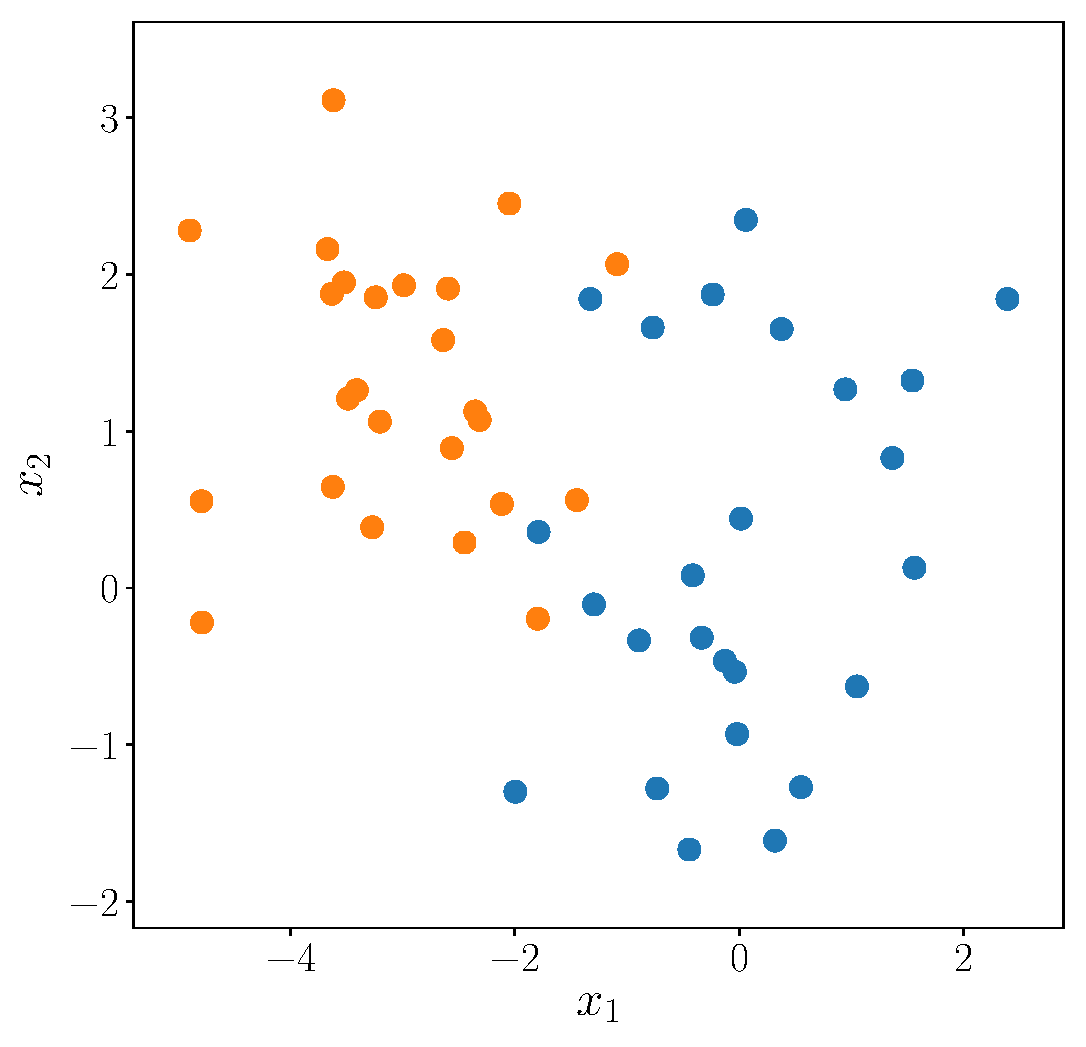
\includegraphics[width=0.35\hsize]{./figures/logistic_regression/logistic_regression_dataset2D}
  \end{figure}
  \begin{itemize}
  \item Supervised learning setting with inputs $\vec x_n\in\R^D$ and
    \cemph{binary} targets $y_n\in\{0,1\}$ belonging to
    \cemph{classes} $\class_1, \class_2$.
  \item Objective:
    \begin{itemize}
    \item Given new test input $\vx_n^*$, predict the label $y_n^*$.
    \item Find a decision boundary\slash surface that separates the two classes
    \end{itemize}
  \end{itemize}
  
\end{frame}






\begin{frame}{Class Posteriors}
  \begin{itemize}
  \item Binary classification problem with two classes $\class_1, \class_2$. \pause
  \item Posterior class probability $p(y=1|\vec x) = p(\class_1|\vec x)$:
    \begin{align*}
      p(\class_1|\vec x) &= \frac{p(\vec x|\class_1)p(\class_1)}{p(\vec
                           x)}\,,\\
      p(\vec x) &= p(\vec x|\class_1) p(\class_1) + p(\vec x|\class_2)p(\class_2)
    \end{align*}
  \end{itemize}

\pause

\arrow Learning from data requires figuring out what $p(\vx\given\class_c)$ is from data.
\end{frame}


\begin{frame}{Generative modelling}
  \begin{figure}
    \centering
    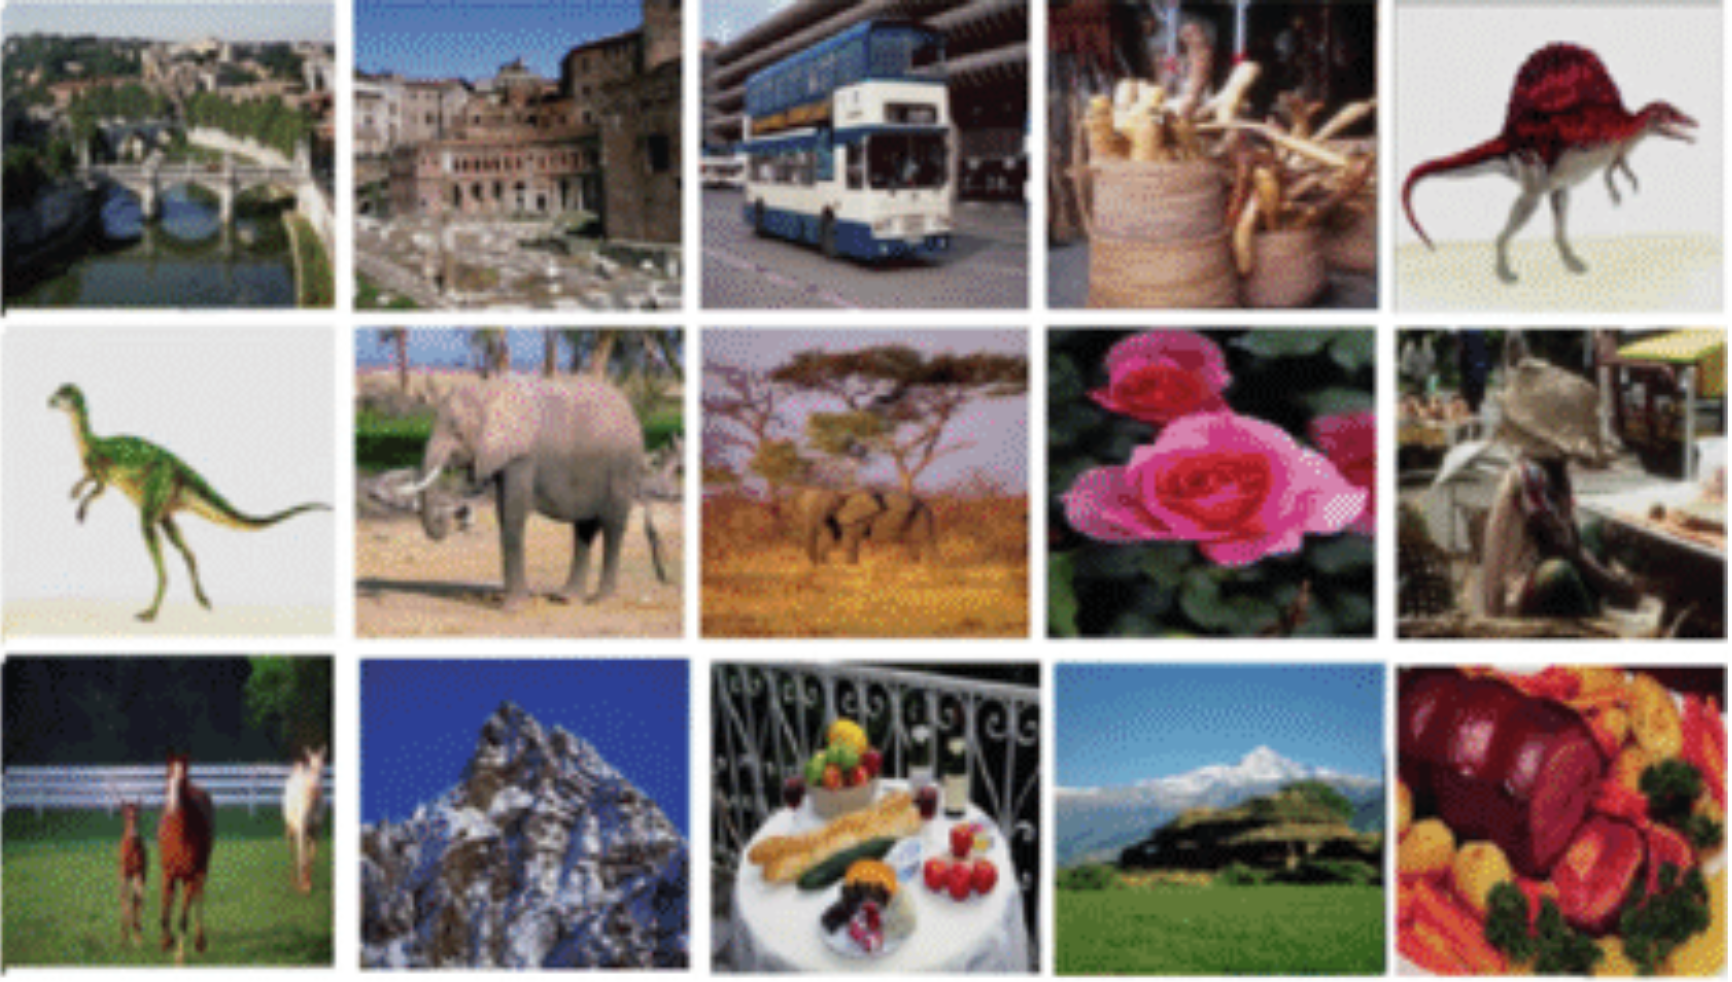
\includegraphics[height=4cm]{./figures/logistic_regression/imagenet}
  \end{figure}
  \begin{itemize}
  \item Inputs can be high-dimensional (e.g.~images)
  \item $p(\vx\given\class_c)$ can be very complicated
  \end{itemize}
  \pause
  \begin{center}
    Imagine learning how to create photorealistic images before being able to recognise them!
  \end{center}
\end{frame}





\begin{frame}{Density ratios}
  We only need the \emph{ratio of weighted likelihoods}
  \begin{align*}
    p(\class_1|\vec x) &= \frac{p(\vec x|\class_1)p(\class_1)}{p(\vec x|\class_1) p(\class_1) + p(\vec x|\class_2)p(\class_2)}\,,\\
                       &= \frac{1}{1 + \frac{p(\vec x|\class_2)p(\class_2)}{p(\vec x|\class_1)p(\class_1)}}\,,
                       % a := \log \frac{p(\class_1|\vec x)}{p(\class_2|\vec x)} =
                       % \log\frac{p(\vec x|\class_1)p(\class_1)}{p(\vec x|\class_2)p(\class_2)}
  \end{align*}

  \pause
  
  Idea: Instead of learning $p(\vx\given\class_c)$, can we just learn $\frac{p(\vec x|\class_2)p(\class_2)}{p(\vec x|\class_1)p(\class_1)}$? \pause
  \begin{gather}
    p(\class_1\given \vx, r(\cdot)) = \frac{1}{1 + r(\vx)} \qquad \text{with } r: \Reals^D \to \Reals^+ \,.
  \end{gather}

  \pause

  Positive functions are a pain... Let's take logs to use $f: \Reals^D\to\Reals$:
  \begin{gather}
    p(\class_1\given \vx, f(\cdot)) = \underbrace{\frac{1}{1 + \exp (-f(\vx))}}_{\text{Logistic sigmoid } \sigma(f(\vx))}
  \end{gather}
\end{frame}


\begin{frame}{Logistic Sigmoid}
  \begin{figure}
    \centering
    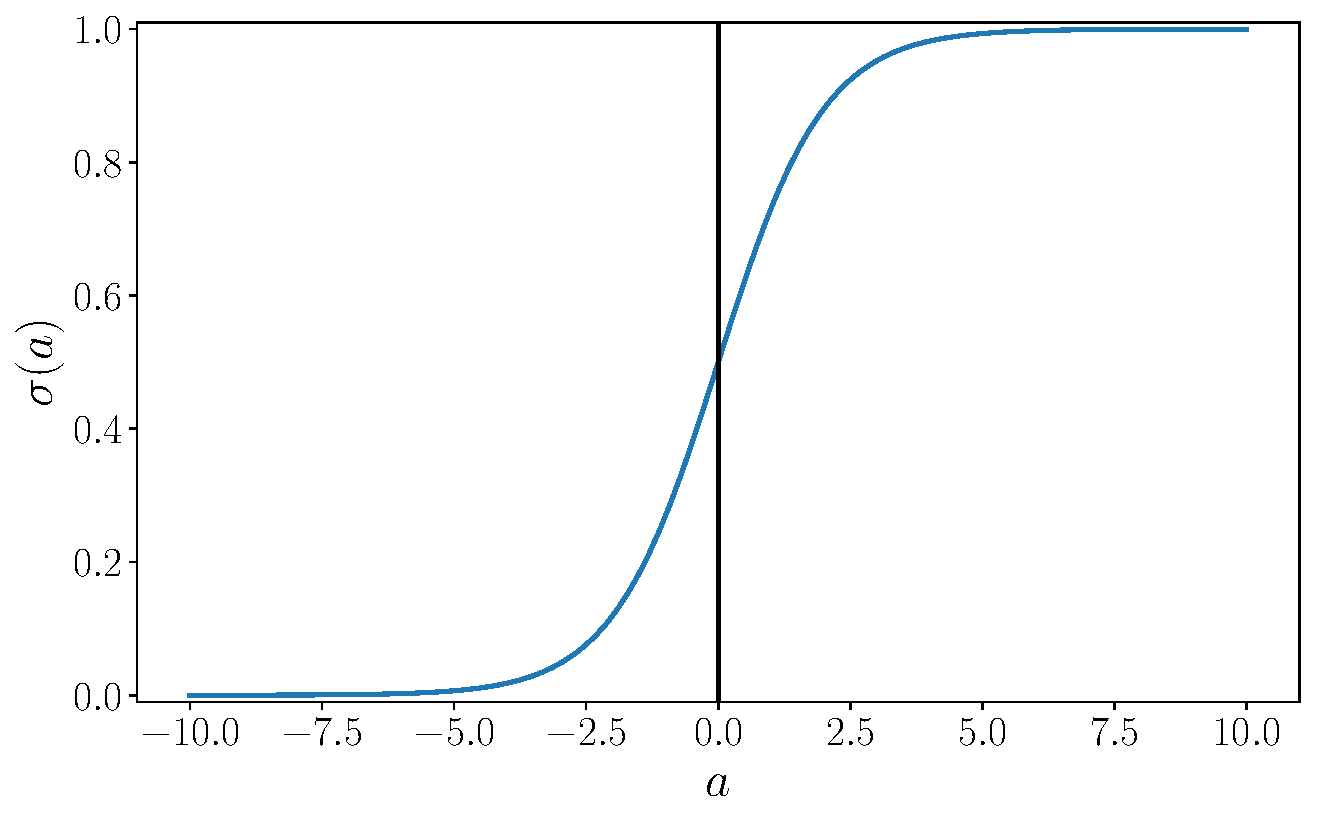
\includegraphics[width=0.5\hsize]{./figures/logistic_regression/sigmoid}
  \end{figure}
  %
  \begin{align*}
    f(\vx) &:= \log \frac{p(\class_1|\vec x)}{p(\class_2|\vec x)} =
        \log\frac{p(\vec x|\class_1)p(\class_1)}{p(\vec
        x|\class_2)p(\class_2)}\\
    \sigma(f(\vx))&:=\frac{1}{1+\exp(-f(\vx))} =  p(\class_1|\vec x)
    % \\
    % \sigma(-a) &= 1-\sigma(a)\\
    % a &= \log\big(\frac{\sigma}{1-\sigma}\big) \quad \text{\emph{Logit function}}
  \end{align*}
\end{frame}


\begin{frame}{What type of function should $f(\cdot)$ be?}
  \begin{itemize}
  \item Assume \cemph{Gaussian class conditionals}
    \begin{align*}
      p(\vec x |\class_k) = \gaussx{\vec x}{\vec\mu_k}{\mat\Sigma}
    \end{align*}
    where the \cemph{covariance matrix $\mat\Sigma$ is shared} across all $K$
    classes.
    \pause
  \item For $K=2$ we get (Bishop, 2006)\nocite{Bishop2006}
    \begin{align*}
      &p(\class_1|\vec x) = \sigma(\vec\theta\T \vec x +
      \theta_0)\,,\\
      &\vec\theta := \mat\Sigma\inv(\vec\mu_1 -\vec\mu_2)\,,\quad 
      \theta_0 := \frac{1}{2} \Big(\vec \mu_2\T  \mat\Sigma\inv  \vec \mu_2-\vec\mu_1\T \mat\Sigma\inv \vec\mu_1\Big )  
       + \log\frac{p(\class_1)}{p(\class_2)}% \frac{1}{2}(\vec\mu_2 -
      % \vec\mu_1)\T\mat\Sigma\inv(\vec\mu_2 - \vec\mu_1) +
      %   \log\frac{p(\class_1)}{p(\class_2)}\\
    \end{align*}
    % \arrow Linear in $\vec x$\\
    \pause
    \hspace{-1mm}\arrow Argument of the sigmoid is linear in $\vec x$\\
    \pause
    \arrow Decision boundary is a surface along which the posterior
    class probabilities $p(\class_k|\vec x)$ are constant\\
    \arrow \emph{Decision boundary is a linear function of $\vec x$}
    \pause
      \item If covariances are not shared: Quadratic decision boundaries
  \end{itemize}
\end{frame}



\begin{frame}{Classifying from data samples}
One approach (generative):
\begin{enumerate}
\item Define priors over two Gaussian distributions for $p(\vx\given\class_c)$
\item Given data, find posteriors over Gaussians
\item Given our beliefs over $p(\vx\given\class_c)$, apply Bayes' rule to get $p(\class_c\given\vx)$
\end{enumerate}

\pause 

\vspace{0.4cm}

Alternative approach (discriminative):
\begin{enumerate}
\item Define prior on linear functions for $f(\cdot)$
\item Given data, find posterior over $f(\cdot)$, which directly translates to $p(\class_c\given\vx)$
\end{enumerate}
\end{frame}




\begin{frame}{Classifying from data samples}
One approach:
\begin{enumerate}
\item Define priors over two \emph{general} distributions for $p(\vx\given\class_c)$
\item Given data, find posteriors over \emph{distributions}
\item Given our beliefs over $p(\vx\given\class_c)$, apply Bayes' rule to get $p(\class_c\given\vx)$
\end{enumerate}

\vspace{0.4cm}

Alternative approach:
\begin{enumerate}
\item Define prior on \emph{general, non-linear} functions for $f(\cdot)$
\item Given data, find posterior over $f(\cdot)$, which directly translates to $p(\class_c\given\vx)$
\end{enumerate}
\end{frame}






\begin{frame}{Model Specification -- Logistic regression}
  \begin{itemize}
  \item \onslide+<2->{Bernoulli} likelihood
    \vspace{-5mm}
    \begin{columns}
      \column{0.55\hsize}
      \onslide+<2->{
    \begin{align*}
      &y\in\{0,1\}\\
      &p(y|\vec x, \vec\theta) = \Ber(y|\mu(\vec x))\,,\\
      &\mu(\vec
        x) = p(y=1|\vec x) = \sigma(\vec\theta\T\vec x)
    \end{align*}
    }
    \column{0.45\hsize}
    % \vspace{-8mm}
      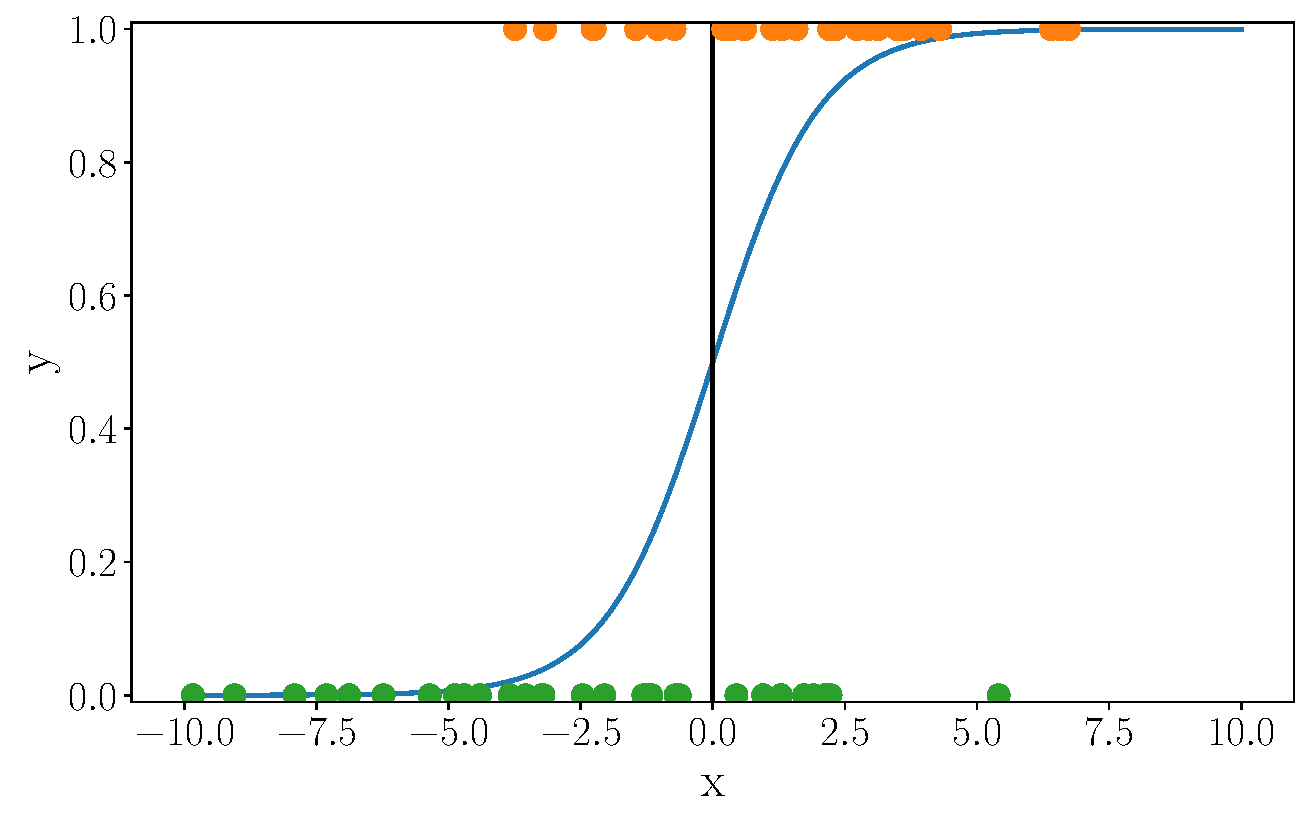
\includegraphics[width=\hsize]{./figures/logistic_regression/sigmoid_with_data}
    \end{columns}
    \onslide+<3->{
\item Label $y$ depends on input location $\vec x$, i.e., $\mu(\vec
  x)$ needs to be a function of $\vec x$
}
\onslide+<4->{
  \item Idea: Linear model $\vec\theta\T\vec x$ (as in linear
    regression)
  }
  \onslide+<5->{
  \item Ensure $0\leq \mu(\vec x) \leq 1$
  }
  \onslide+<6->{
  \item Squash the linear combination through a function that
    guarantees this:
    \vspace{-7mm}
    \begin{align*}
      &\mu(\vec x) = \sigma(\vec\theta\T\vec x)\\
      \implies      &p(y|\vec x, \vec\theta) = \Ber(y|\sigma(\vec\theta\T\vec x))
    \end{align*}
    }
  \end{itemize}
  
\end{frame}


\begin{frame}{Model fitting}
Model is very similar to \emph{linear regression}, but with a different \emph{likelihood}.
\pause
\begin{itemize}
\item Can we find the posterior?
\begin{align}
p(\vtheta\given X, \vy) &= \frac{\prod_{n=1}^N p(y_n\given \sigma(\vtheta\transpose\vx)) p(\vtheta)}{p(\vy\given X)}
\end{align} \pause
\item Can we find the predictive distribution?
\begin{align}
p(y^*\given X, \vy, \vx^*) &= \int p(y^*\given \vtheta, \vx^*) p(\vtheta\given X, \vy) \calcd{\vtheta}
\end{align}
\end{itemize}
\end{frame}


\begin{frame}{Logistic regression posterior}
\begin{align}
p(\vtheta\given X, \vy) &= \frac{\prod_{n=1}^N p(y_n\given \sigma(\vtheta\transpose\vx)) p(\vtheta)}{p(\vy\given X)} \\
&= \frac{1}{p(\vy\given X)} \prod_{n=1}^N \text{Ber}(y_n|\sigma(\vtheta\transpose\vx)) \NormDist{\vtheta; 0, v\mathbf{I}} \,, \\
p(\vy\given X) &= \int p(\vy\given X, \vtheta) p(\vtheta) \calcd{\vtheta} \,.
\end{align}
\pause
Problem 1: \pause
\begin{enumerate}
\item No closed-form solution for the marginal likelihood \pause
\item Can only evaluate the posterior up to a constant
\end{enumerate}
\end{frame}



\begin{frame}{Logistic regression predictive distribution}
  \begin{align}
    p(y^*\given X, \vy, \vx^*) &= \int p(y^*\given \vtheta, \vx^*) p(\vtheta\given X, \vy) \calcd{\vtheta} \\
&= \frac{1}{p(\vy\given X)} \int p(y^*\given \vtheta,\vx^*) \,\cdot \nonumber \\ 
&\qquad\qquad\qquad\prod_{n=1}^N\text{Ber}(y_n|\sigma(\vtheta\transpose\vx)) \NormDist{\vtheta; 0, v\mathbf{I}} \calcd{\vtheta}
  \end{align}
\pause
Problem 2: \pause
\begin{itemize}
\item No closed-form solution to integral (similar to marginal likelihood)
\item Also need to normalise by the marginal likelihood
\end{itemize}
\end{frame}


\begin{frame}{Point Estimate}
  \begin{itemize}
  \item Estimate model parameters $\vec\theta$ as a point, not a distribution (MLE or MAP)
    \pause
  \item Likelihood (training data $\mat X, \vec y$):
    \begin{align*}
      p(\vec y|\mat X, \vec\theta) &=
                                     \prod_{n=1}^N\Ber(y_n|\sigma(\vec\theta\T\vec 
                                     x_n))=\prod_{n=1}^N(\sigma(\vec\theta\T\vec
                                     x_n))^{y_n}(1-\sigma(\vec\theta\T\vec x_n))^{1-y_n}\\
                                   &= \prod_{n=1}^N\mu_n^{y_n}(1-\mu_n)^{1-y_n}\\
      \mu_n &:= \sigma(\vec\theta\T\vec x_n)
    \end{align*} \pause \vspace{-0.4cm}
  \item Minimise \emph{negative log likelihood (cross-entropy):}
    \pause
    \begin{align*}
     NLL &=  -\sum_{n=1}^N y_n\log\mu_n + (1-y_n)\log(1-\mu_n)
    \end{align*}
  % \item Alternatively, if $y\in{\pm 1}$ we can write the cross entropy
  %   as
  %   \begin{align*}
  %     \sum_{n=1}^N\log\big(1+\exp(-y_n\vec\theta\T\vec x_n)\big)
        %       \end{align*}
  \end{itemize}
\end{frame}



\begin{frame}{Model Fitting (2)}
  \begin{itemize}
    \item Derivative of sigmoid w.r.t. its argument:
  \begin{align*}
    &\sigma(z_n) = \frac{1}{1+\exp(-z_n)}\\
    &\implies \diffF{\sigma(z_n)}{z_n} = \onslide+<2->{\frac{\exp(-z_n)}{(1+\exp(-z_n))^2}=\sigma(z_n)(1-\sigma(z_n))}
  \end{align*}
  \onslide+<3->{
  \item Gradient of the negative log-likelihood:
  \begin{align*}
   \diffF{NLL}{\vec\theta} &= -\sum_{n=1}^N\left(y_n
                             \frac{1}{\mu_n} -
                             (1-y_n)\frac{1}{1-\mu_n}\right)  \colchar{$\displaystyle\diffF{\mu_n}{\vec\theta}$}{orange}
                             %\colchar{$\displaystyle\diffF{\mu_n}{\vec\theta}$}{orange}
    \\
 \colchar{$\displaystyle\diffF{\mu_n}{\vec\theta}$}{orange}
                           &=
                             \onslide+<4->{
                             \diffF{}{\vec\theta}\sigma(\underbrace{\vec\theta\T\vec
                             x_n}_{z_n})  =
                             \diffF{\sigma(z_n)}{z_n}\diffF{z_n}{\vec\theta}
                             = \sigma(z_n)(1-\sigma(z_n))\vec x_n\T
                             }
  \end{align*}
  }
\end{itemize} 
\end{frame}
%%%%%%%%%%%%% 
\begin{frame}{Model Fitting (3)}
  \begin{align*}
    \diffF{NLL}{\vec\theta} = (\vec\mu - \vec y)\T\mat X\\
    \mat X = [\vec x_1, \dotsc, \vec x_N]\T
  \end{align*}

  \begin{itemize}
  \item \calert{No closed-form solution} \arrow Gradient descent methods
  \item \cemph{Unique global optimum exists} (NLL) is \emph{convex}.
  \end{itemize}

  \begin{gather}
    p(\vtheta\given \mat X, \vy) \approx \delta(\vtheta - \vtheta^*) \\
    \vtheta^* = \argmax_\theta \log p(\vy\given \mat X, \vtheta) + \log p(\vtheta)
  \end{gather}
\end{frame}


%%%%%%%%%%%%%
\begin{frame}{Maximum likelihood solution}
  \begin{figure}
    \centering
    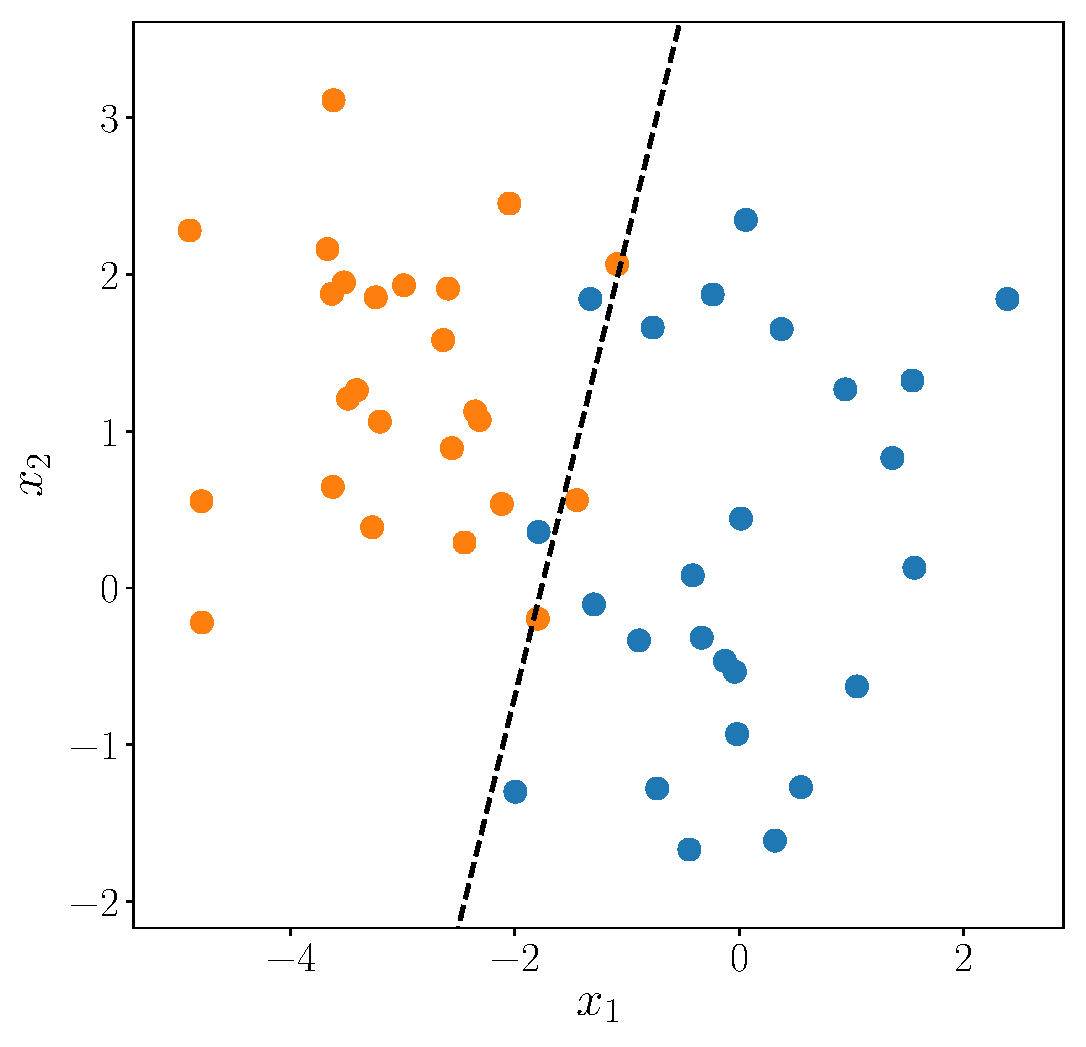
\includegraphics[width=0.5\hsize]{./figures/logistic_regression/logistic_regression_mle_2d}
  \end{figure}

  \begin{align*}
    p(y|\vec x, \vec\theta)  = \Ber(\sigma(\theta_0 + \theta_1x_1 + \theta_2x_2))
  \end{align*}
\end{frame}

%%%%%%%%%%%%%
\begin{frame}{Comments on Maximum Likelihood}

  \begin{itemize}
    \item If the classes are linearly separable, the decision boundary
      is \cemph{not unique} and the predictions will become extreme
    \item \calert{Overfitting} is a again a problem when we work with features
      $\vec\phi(\vec x)$ instead of $\vec x$ (or a GP for that matter)
    \item Maximum a posteriori estimation can address these issues to
      some degree
  \end{itemize}
\end{frame}



%%%%%%%%%%%%%
\begin{frame}{MAP Solution}

  \begin{figure}
    \centering
    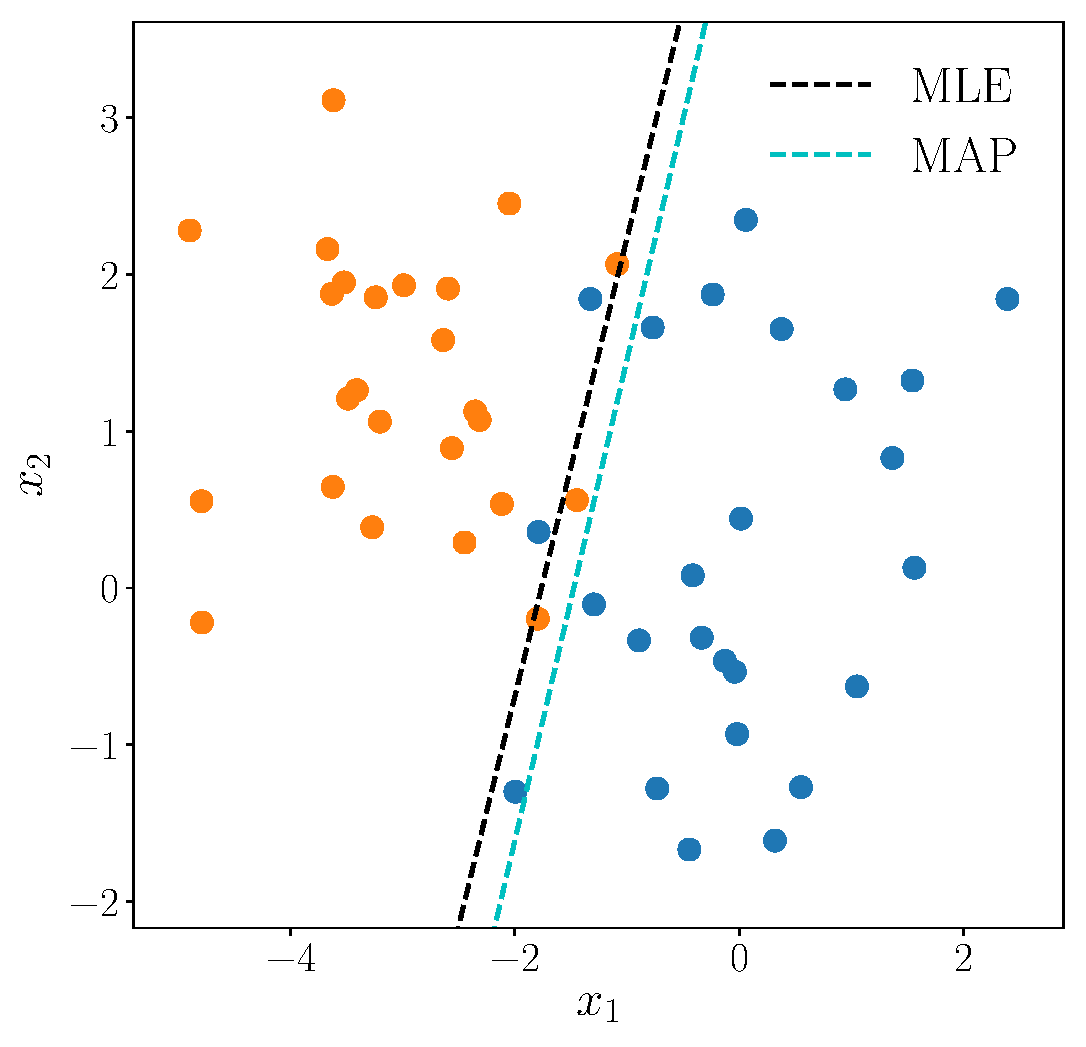
\includegraphics[width=0.45\hsize]{./figures/logistic_regression/logistic_regression_2D_mle_map}
  \end{figure}
  \vspace{-5mm}
  \begin{itemize}
    \item Log-posterior:
  \begin{align*}
    \log p(\vec\theta |\mat X, \vec y) = \log p(\vec y|\mat X,
    \vec\theta) + \log p(\vec\theta) + \text{ const}
  \end{align*}
\item \calert{No closed-form solution} for $\vec\theta_{\text{MAP}}$ \\\arrow
  \cemph{Numerical maximization of the log-posterior}
  \end{itemize}
\end{frame}


%%%%%%%%%%%%%%%%%%%%
\begin{frame}{Predictive Labels}

  \begin{figure}
    \centering 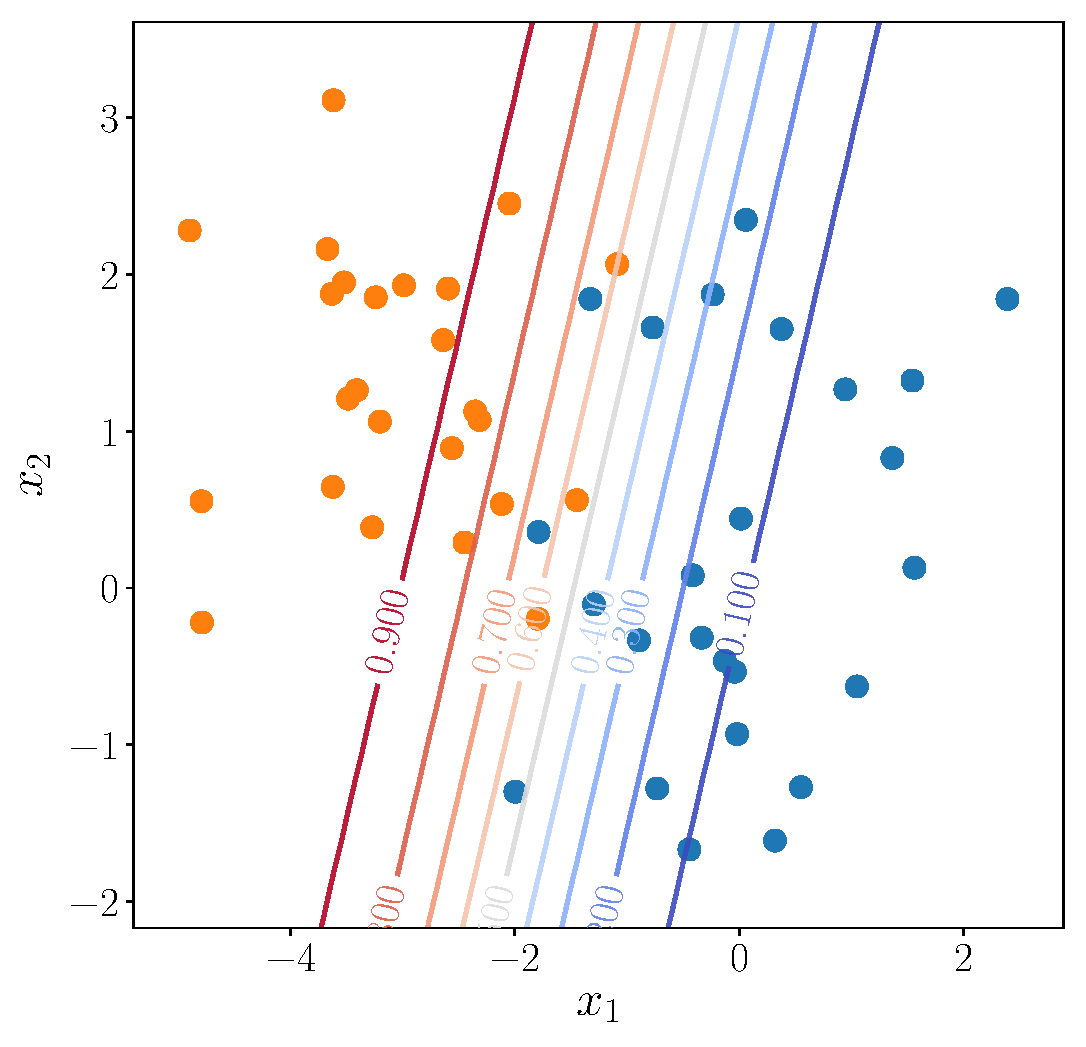
\includegraphics[width
    =0.5\hsize]{./figures/logistic_regression/logistic_regression_map_prediction}
  \end{figure}

  \begin{align*}
    p(y=1|\vec x, \vec\theta_{\text{MAP}}) = \Ber(\sigma(\vec x\T\vec\theta_{\text{MAP}})
  \end{align*}
\end{frame}


\section{Laplace Approximation}


\begin{frame}{Approximate Inference}
If we can't do the required integrals exactly, \\ ... can we approximate them?
\begin{itemize}
\item The true posterior is intractable
\item Can we find a manageable distribution that is close?
\end{itemize}

\vspace{0.5cm}

\pause
\begin{center}Gaussian distributions are manageable, \\
so can we find a Gaussian approximation?
\end{center}

\end{frame}


\begin{frame}[t]{Laplace Approximation}
For a distribution $p(\vx) = \frac{1}{Z} \tilde{p}(\vx)$
\begin{itemize}
\item Maximising $\tilde p(\vx)$ gives us the mode $\vx^*$
\item Can we find an approximation to the variance? \pause \\
\arrow 2nd order Taylor-series approximation
\end{itemize}
\pause
\only<1,2>{
\vspace{2.6cm}
}
\only<3>{
\begin{gather*}
\log {p}(\vx) \approx -\log Z + \log\tilde{p}(\vx^*) + \mathbf{J}(\vx^*)(\vx-\vx^*) + \frac{1}{2}(\vx - \vx^*)\transpose\mat H(\vx^*)(\vx-\vx^*) \\
\mathbf{J}\text{ : \hspace{0.3cm} Jacobian, \hspace{0.5cm} }\mathbf{H}\text{ : Hessian.} \nonumber
\end{gather*}
}
\onslide<4->{
\begin{gather*}
\log {p}(\vx) \approx -\log Z + \log\tilde{p}(\vx^*) + \cancelto{0}{\mathbf{J}(\vx^*)(\vx-\vx^*)} + \frac{1}{2}(\vx - \vx^*)\transpose\mat H(\vx^*)(\vx-\vx^*) \\
\mathbf{J}\text{ : \hspace{0.3cm} Jacobian, \hspace{0.5cm} }\mathbf{H}\text{ : Hessian.} \nonumber
\end{gather*}
Since $\mathbf{J}(\vx^*) = 0$.
}

\onslide<5->{
Equating coefficients with a Gaussian $q(\vx) = \NormDist{\vx; \vmu, \Sigma}$:
\begin{gather}
\vmu = \vx^* \qquad \qquad \Sigma = \mat H(\vx^*)\inv \\
\log Z \approx \log \tilde{p}(\vx) + \frac{D}{2}\log 2\pi + \frac{1}{2}\log \detbar{\mat H(\vx^*)\inv}
\end{gather}
}
\end{frame}



\begin{frame}{Laplace Approximation: Marginal Likelihood}
We can apply the Laplace approximation to approximate a posterior:
\begin{align*}
p(\vx|\vy) &= \frac{\color{OliveGreen}p(\vy|\vx)p(\vx)}{{\color{red} \int} {\color{OliveGreen}p(\vy|\vx)p(\vx)} {\color{red} \calcd \vx}} \Pause \\
&= \frac{1}{\color{red} Z} {\color{OliveGreen} \tilde p(\vx)}
\end{align*} \pause
\begin{itemize}
\item $Z$ is the marginal likelihood!
\end{itemize}
\end{frame}



\begin{frame}[t]{Laplace Approximation: Example}

  \begin{figure}
    \centering 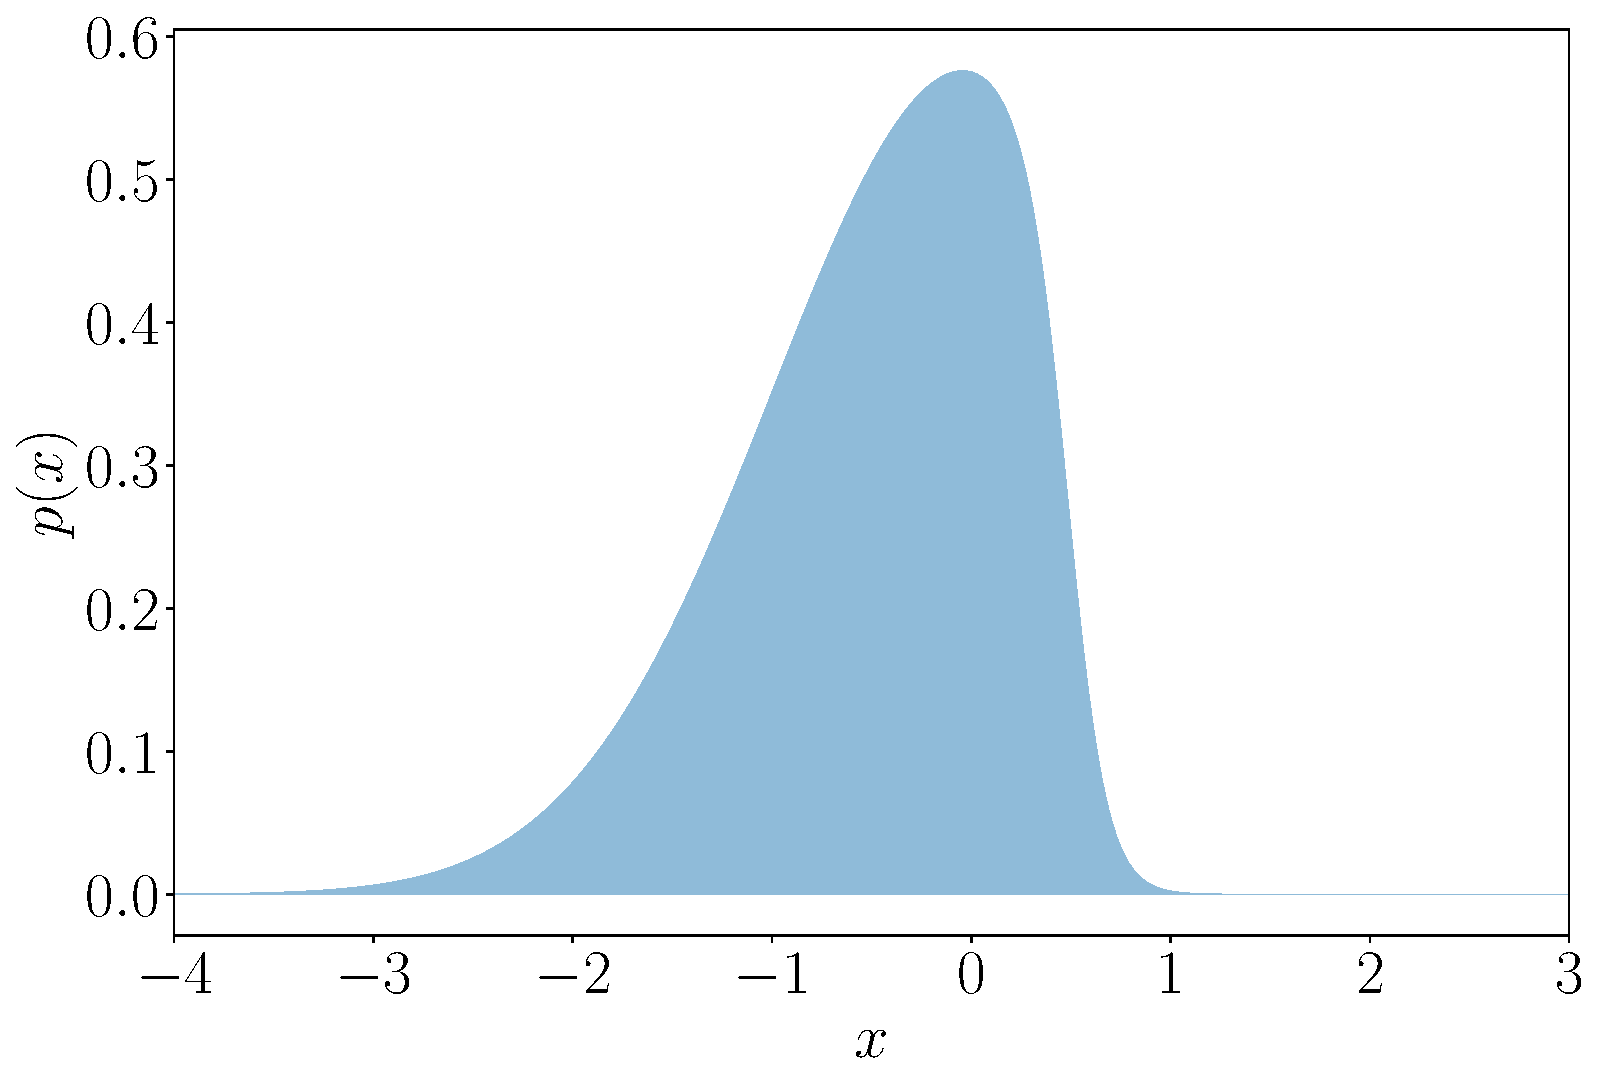
\includegraphics[width=0.4\hsize]{./figures/logistic_regression/laplace_ptilde}
    \onslide+<2->{
      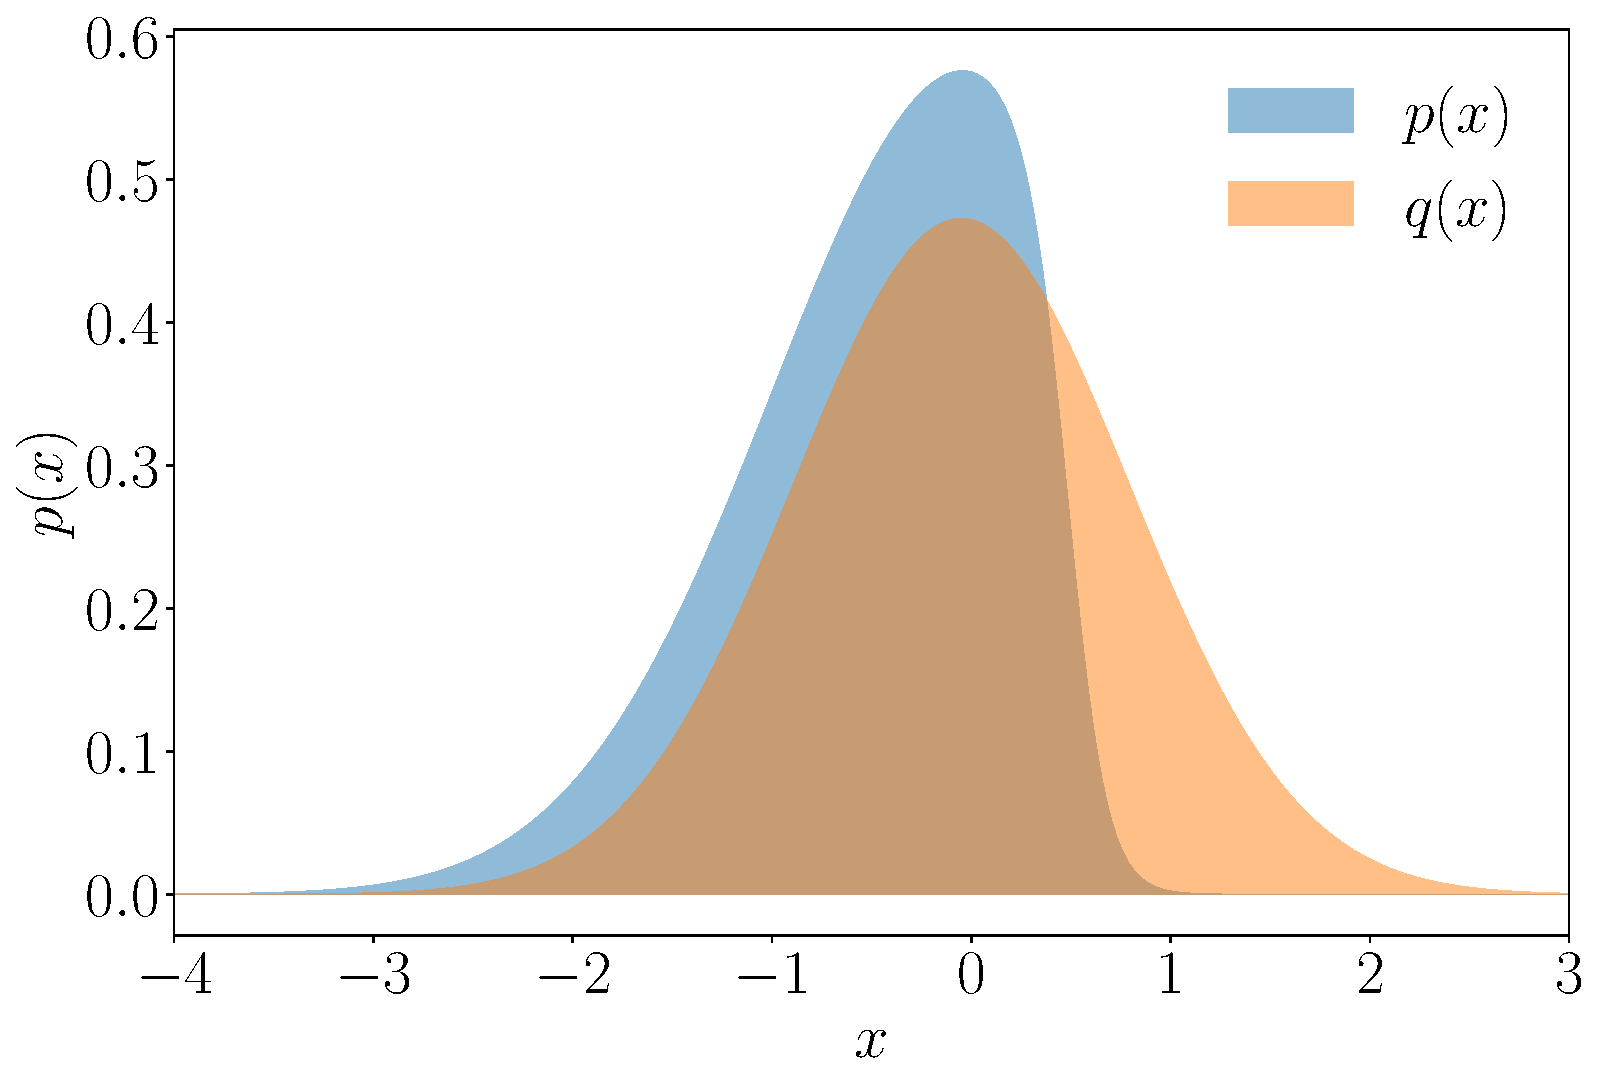
\includegraphics[width=0.4\hsize]{./figures/logistic_regression/laplace_q}
    }
  \end{figure}

  \begin{itemize}
  \item Unnormalized distribution:
    \begin{align*}
      &\tilde p(x) = \exp(-\tfrac{1}{2}x^2)\sigma(ax + b)\\
      \onslide+<2->{&q(x) =  \gaussxBig{x}{x^*}{(1 +a^2 \mu_*(1-\mu_*))^{-1}}\,,\quad \mu_*
      := \sigma(ax_* + b)}
    \end{align*}
    % \begin{align*}
%       \mathrm{Beta}(x|a,b) &~~\propto~~ x^{a-1}(1-x)^{b-1}, \quad a,~b>0\\
% \onslide+<2->{ &\approx \gaussxBig{x}{x^*}{\left(\frac{a-1}{(x^*)^2} + \frac{b-1}{1-(x^*)^2}\right)\inv}}
%     \end{align*}
    
  \end{itemize}
  
\end{frame}




\begin{frame}{Laplace Approximation: Properties}
  \begin{itemize}
  \item Only need to know the \cemph{unnormalized distribution} $\tilde p$
  \item Finding the mode: numerical methods (optimization problem)
  \item \calert{Captures only local properties} of the distribution
  \item Multimodal distributions: Approximation will be different
    depending on which mode we are in (\calert{not unique})
    \pause
  \item For large datasets, we would expect the posterior to converge
    to a Gaussian (Bernstein-von Mises theorem)\\
    \arrow Laplace approximation should work well in this case
  \end{itemize}
\end{frame}



\begin{frame}{Logistic Regression Posterior Approximation}
  \begin{figure}
    \centering
    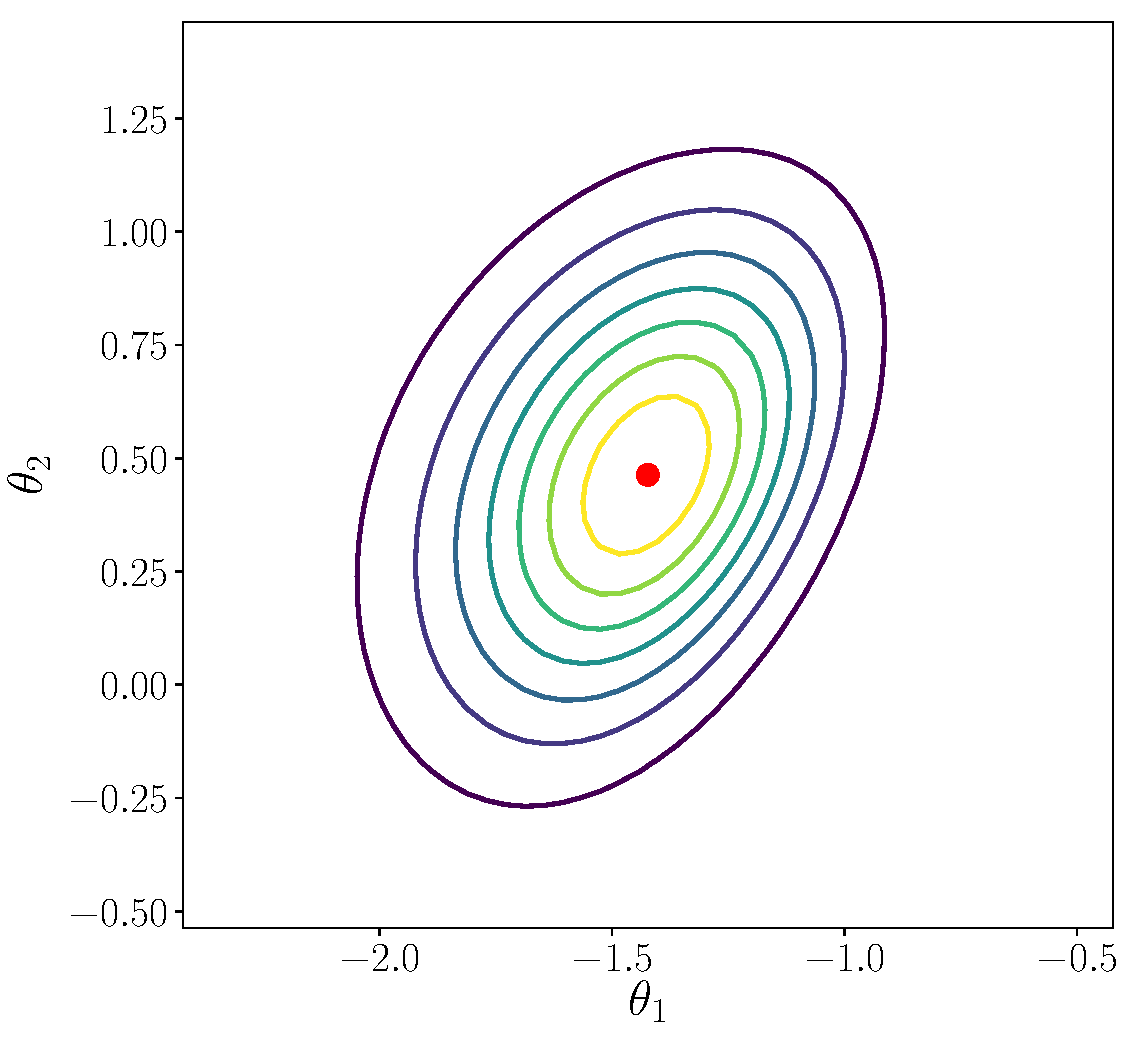
\includegraphics[width=0.45\hsize]{./figures/logistic_regression/logistic_regression_posterior}
    \hspace{5mm}
    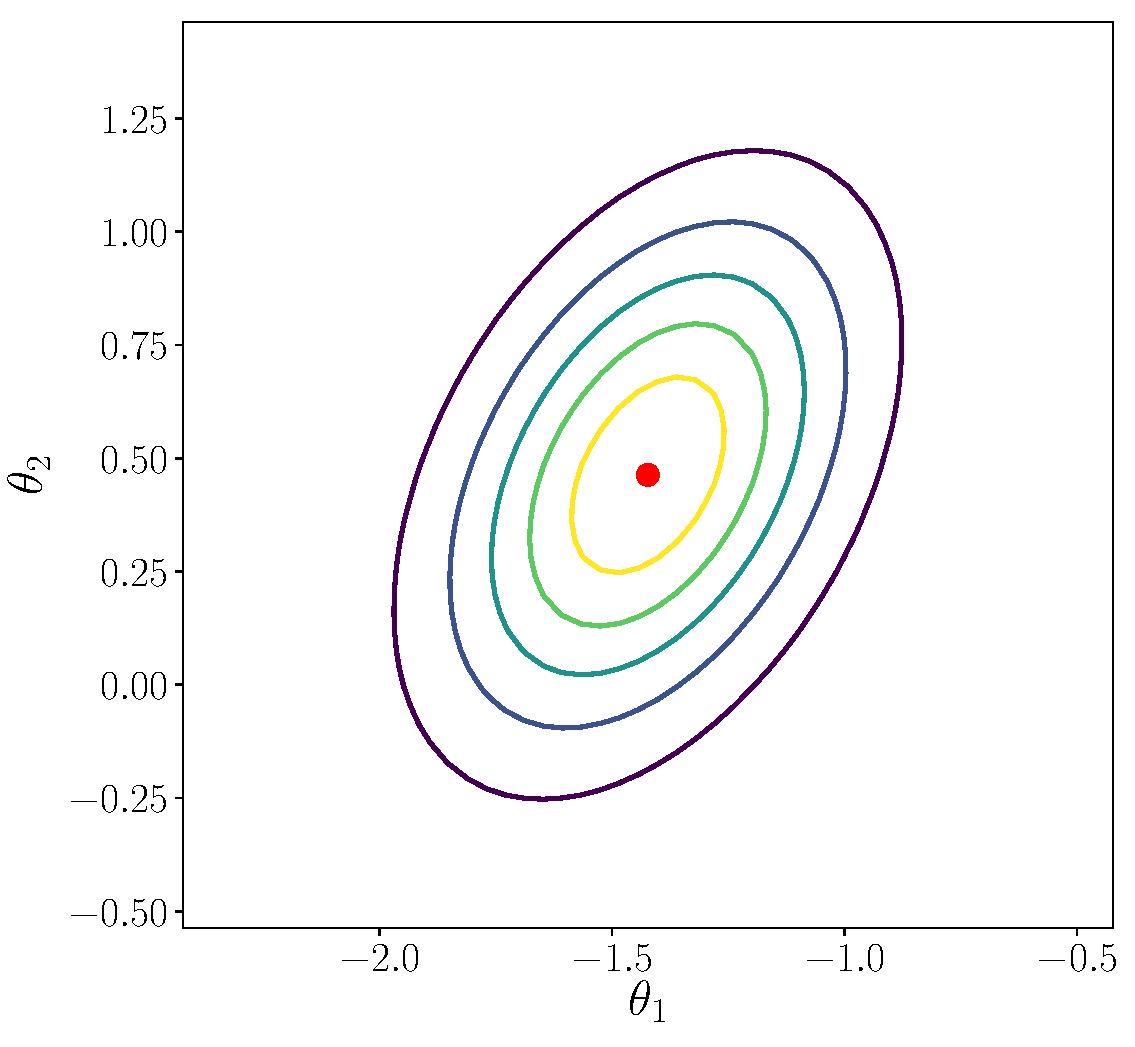
\includegraphics[width=0.45\hsize]{./figures/logistic_regression/logistic_regression_laplace_posterior} 
  \end{figure}

  \begin{itemize}
  \item Left: true parameter posterior
  \item Right: Laplace approximation
  \end{itemize}
  
  
\end{frame}

%%%%%%%%%%%%%%%%%%%%%%%%%%%%%%%%%%%%%%%%%%%%%%
\begin{frame}{Posterior Decision Boundary}

  \begin{figure}
    \centering
    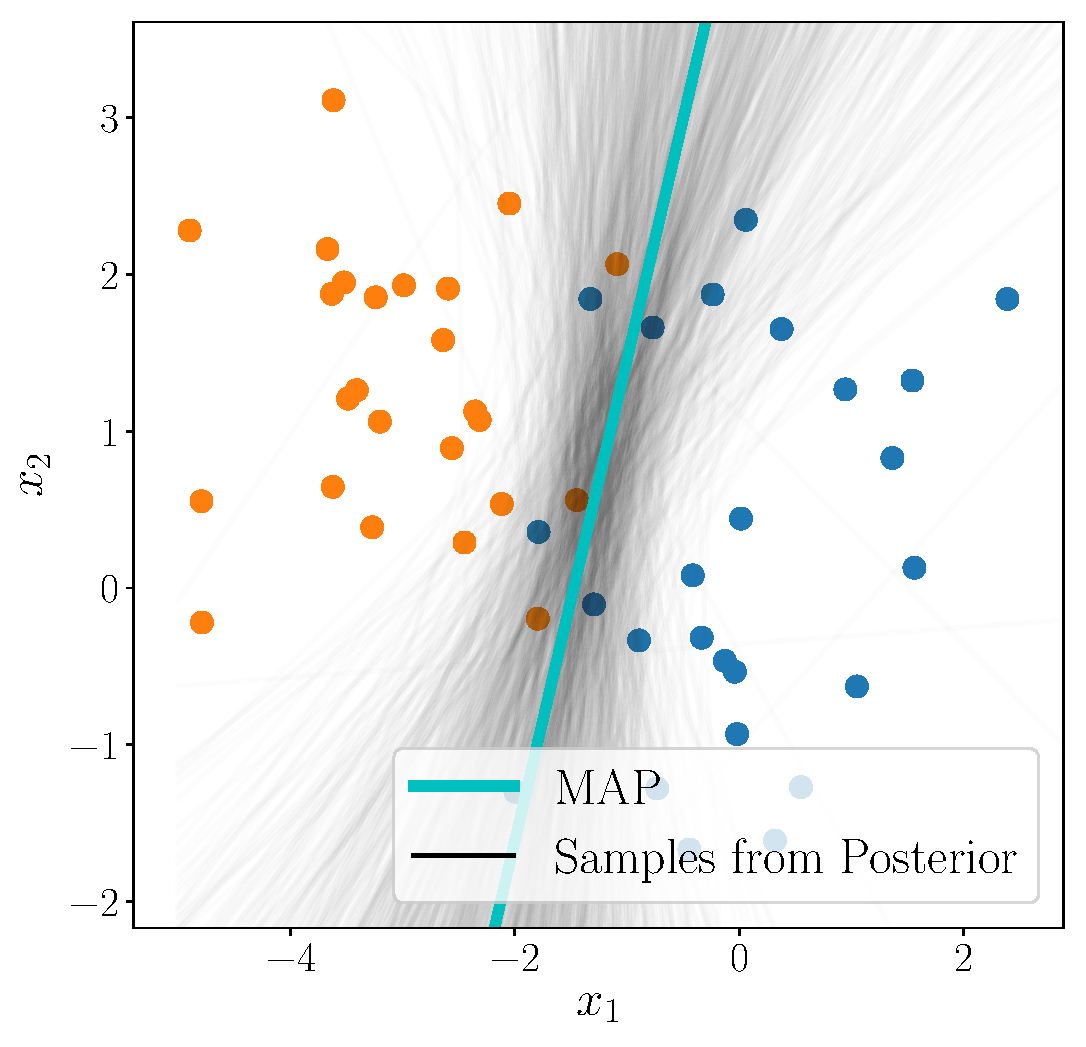
\includegraphics[width=0.45\hsize]{./figures/logistic_regression/logistic_regression_2D_posterior}  
  \end{figure}

  \begin{itemize}
    \item Parameter samples $\vec\theta_i$ drawn from Laplace
      approximation $q(\vec\theta)$ of posterior $p(\vec\theta|\mat X)$
    \item Decision boundary drawn for each $\vec\theta_i$
  \end{itemize}
  
\end{frame}




%%%%%%%%%%%%%%%%%%%%%%%%%%%%%%%%%%%%%%%%%%%%%%


\section{Monte Carlo}


\begin{frame}{Predictions}
  Assume a Gaussian distribution
  $q(\vec\theta)=\gauss{\vec\mu}{\mat\Sigma}$ on the parameters (e.g.,
  Laplace approximation of the posterior). Then:
  \begin{align}
    p(y^*\given X, \vy, \vx^*) &= \int p(y^*\given \vtheta, \vx^*) p(\vtheta\given X, \vy) \calcd{\vtheta} \\
&\approx \int p(y^*\given\vtheta, \vx^*) q(\vtheta) \calcd{\vtheta}
  \end{align}
\pause
\arrow \alert{Integral intractable}
\pause
\arrow Use \emph{Monte Carlo} approximation
\begin{gather}
\int p(y^*\given\vtheta, \vx^*) q(\vtheta) \calcd{\vtheta} \approx \frac{1}{S}\sum_{s=1}^s p(y^*\given\vtheta^{(s)}, \vx^*) \\
\vtheta^{(s)} \sim q(\vtheta)
\end{gather}
\end{frame}


\begin{frame}{Predictions (2)}
  \begin{figure}
    \centering
    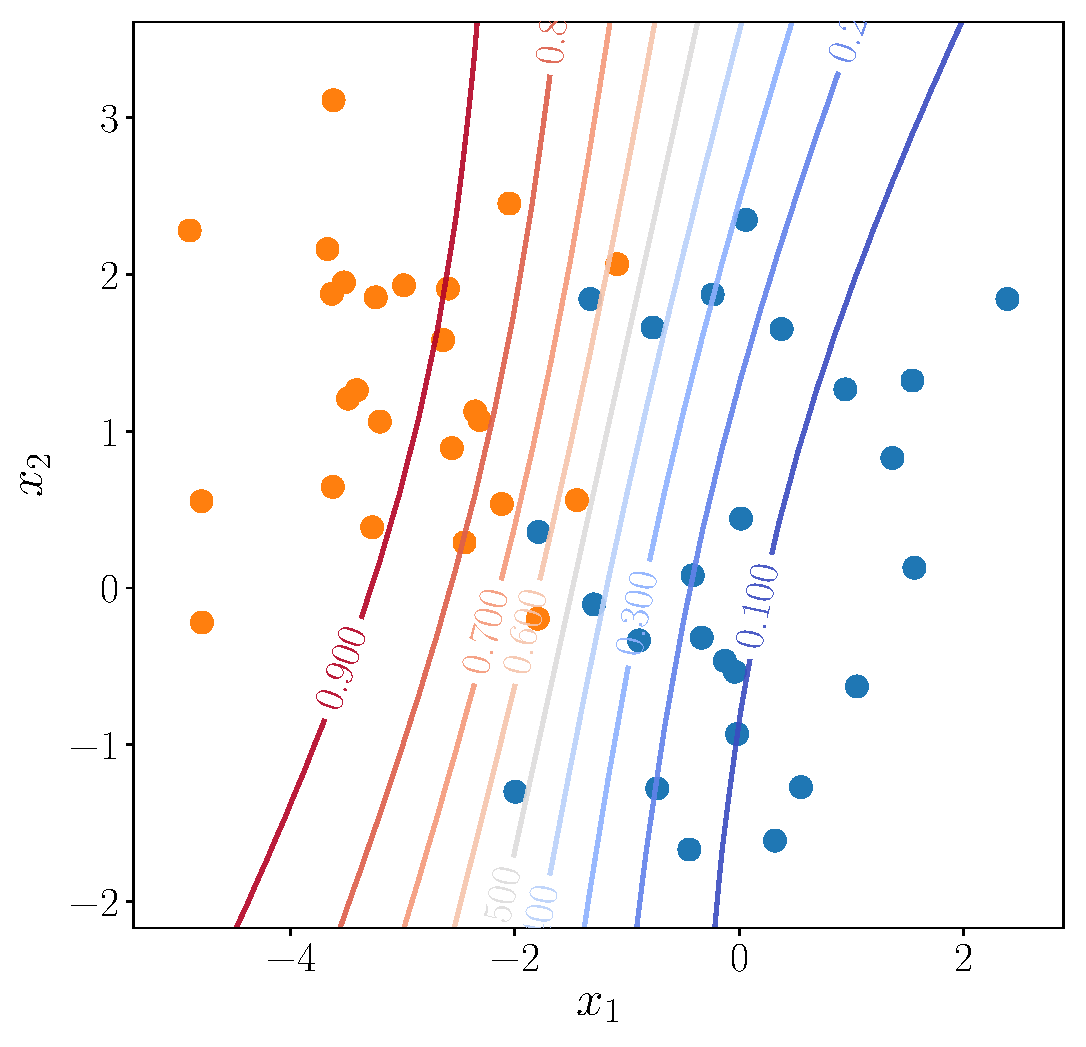
\includegraphics[width=0.5\hsize]{./figures/logistic_regression/logistic_regression_prediction}
  \end{figure}
  \begin{enumerate}
  \item Samples from  Laplace approximation of the posterior
  \item Monte-Carlo estimate of label prediction
  \end{enumerate}
\end{frame}


\begin{frame}{Comparison with MAP Predictions}
  \begin{figure}
    \centering
    \subfloat[MAP]{
          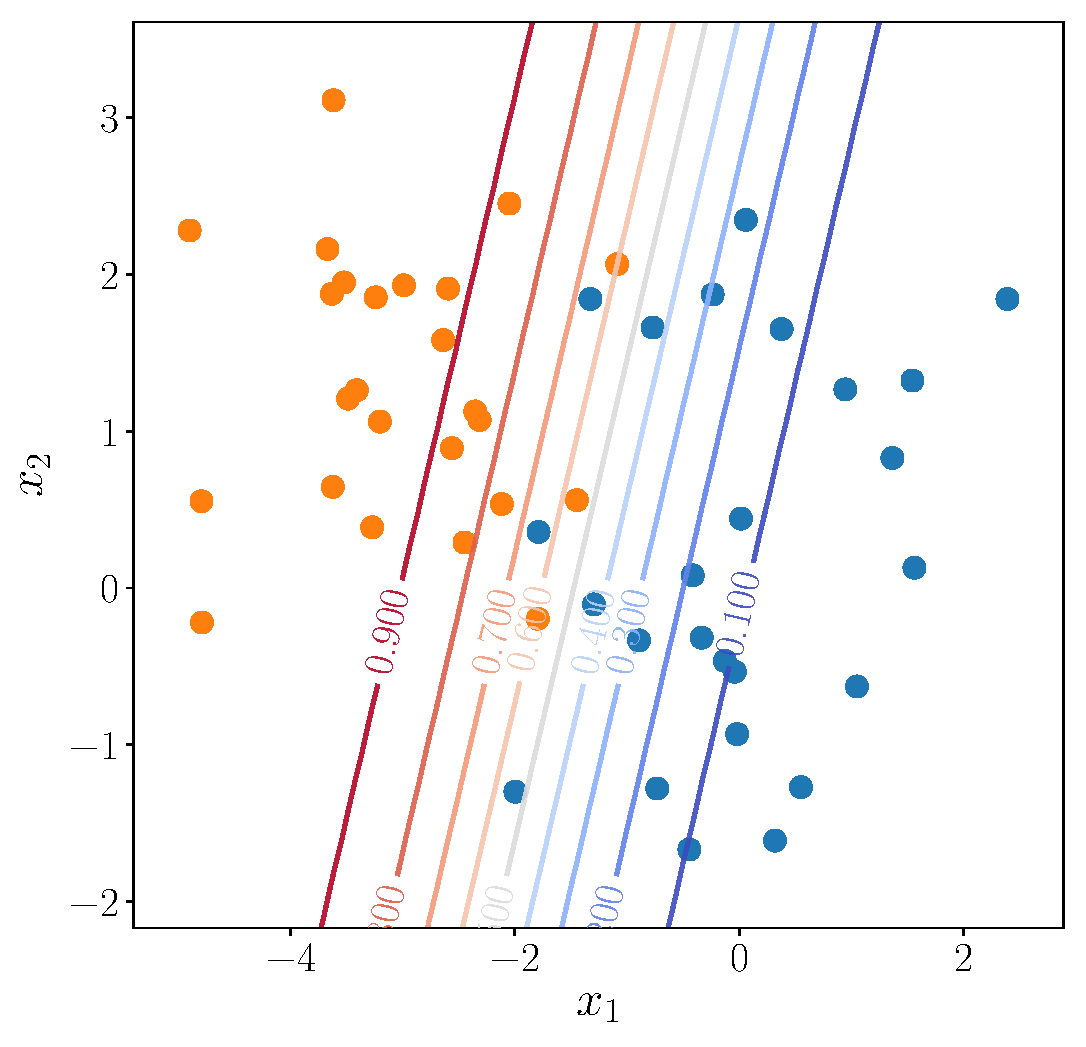
\includegraphics[width=0.45\hsize]{./figures/logistic_regression/logistic_regression_map_prediction}
        }
        \subfloat[Bayesian Logistic Regression]{
          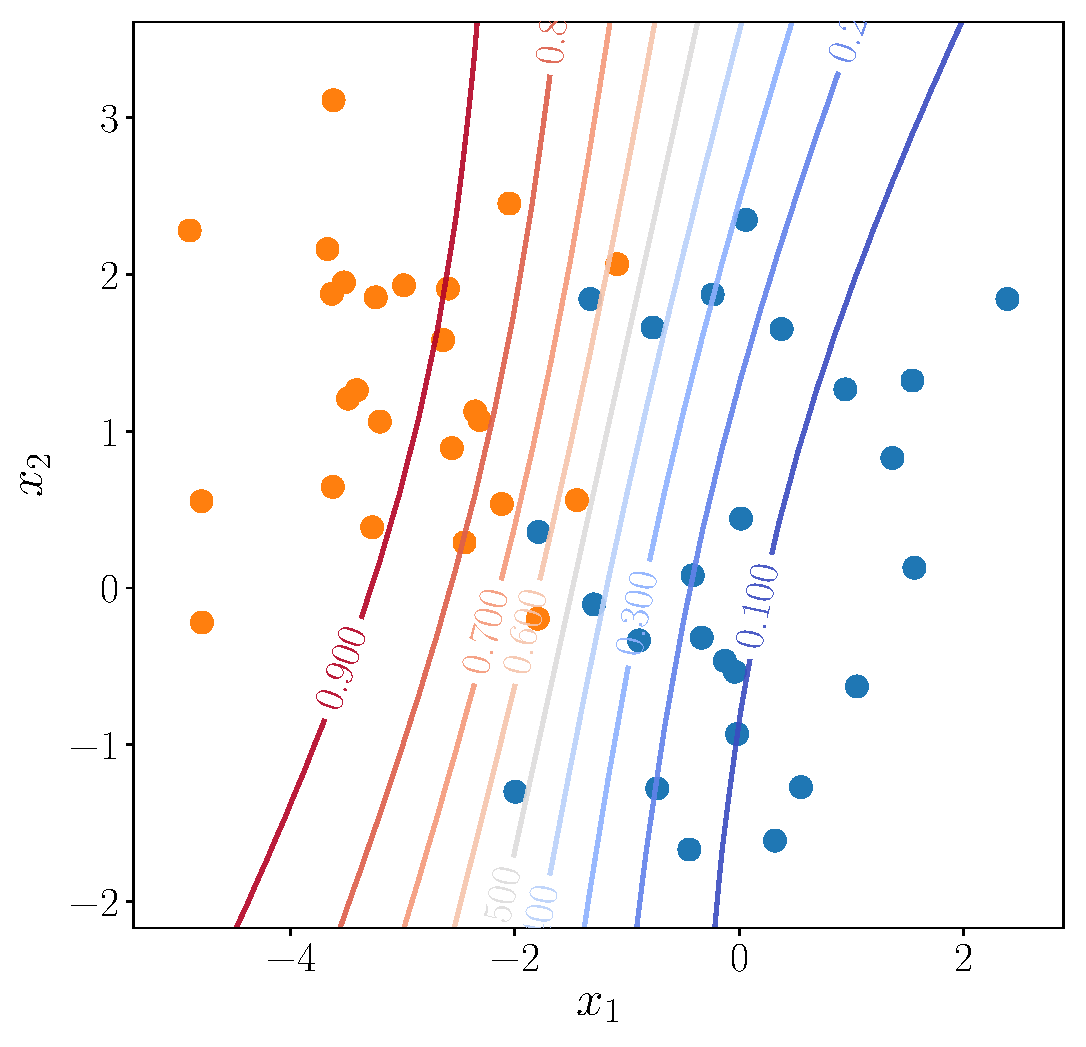
\includegraphics[width=0.45\hsize]{./figures/logistic_regression/logistic_regression_prediction}
    }
  \end{figure}
  \begin{itemize}
    \item Predictive labels
  \end{itemize}
\end{frame}


\begin{frame}{Specifying Monte Carlo Approximations}
A full specification of a MC procedure (e.g.~in an exam) requires:
\begin{itemize}
\item Statement of what is to be computed, e.g.~$\int f(\vx) p(\vx)\calcd \vx$.
\item What we compute in our approximation, e.g.~$\sum_{s=1}^S f(\vx^{[s]})$
\item What distribution we sample from, e.g.~$\vx^{[s]} \sim p(\vx)$.
\item A sentence explaining how we sample from the distribution.
\end{itemize}
\end{frame}


\begin{frame}{Sampling Procedures}
You can assume that we can generate samples from \emph{categorical distributions}\pause, \emph{uniform distributions}\pause, and \emph{standard Normal distributions}. \pause

To generate samples, you can:
\begin{itemize}
\item Reparameterise a distribution. \pause $x = t(\vepsilon)$ (see MML \cite{mml}) \\
 \pause E.g.~Gaussian $\NormDist{\vx; \vmu, \mat K}$
\begin{align}
\vx = \mathrm{chol}(\mat K)\vepsilon + \vmu && \vepsilon \sim \NormDist{0, I_M}
\end{align} \pause
\item Use rejection sampling (later) \pause
\item MCMC (later)
\end{itemize}
\end{frame}



\begin{frame}{Accuracy of MC Estimate}
Remember from MML:
\begin{itemize}
\item As $S\to\infty$, the MC estimate converges to the right value.
\item Variance determines accuracy for finite $S$ (Chebyshev's inequality).
\item Want low variance!
\item Can control this with $S$.
\item Other techniques in future lectures.
\end{itemize}

{\tiny Todo: Make nice notebook illustrating MC estiamte}
\end{frame}




\begin{frame}{Summary}
  \begin{figure}
    \centering
    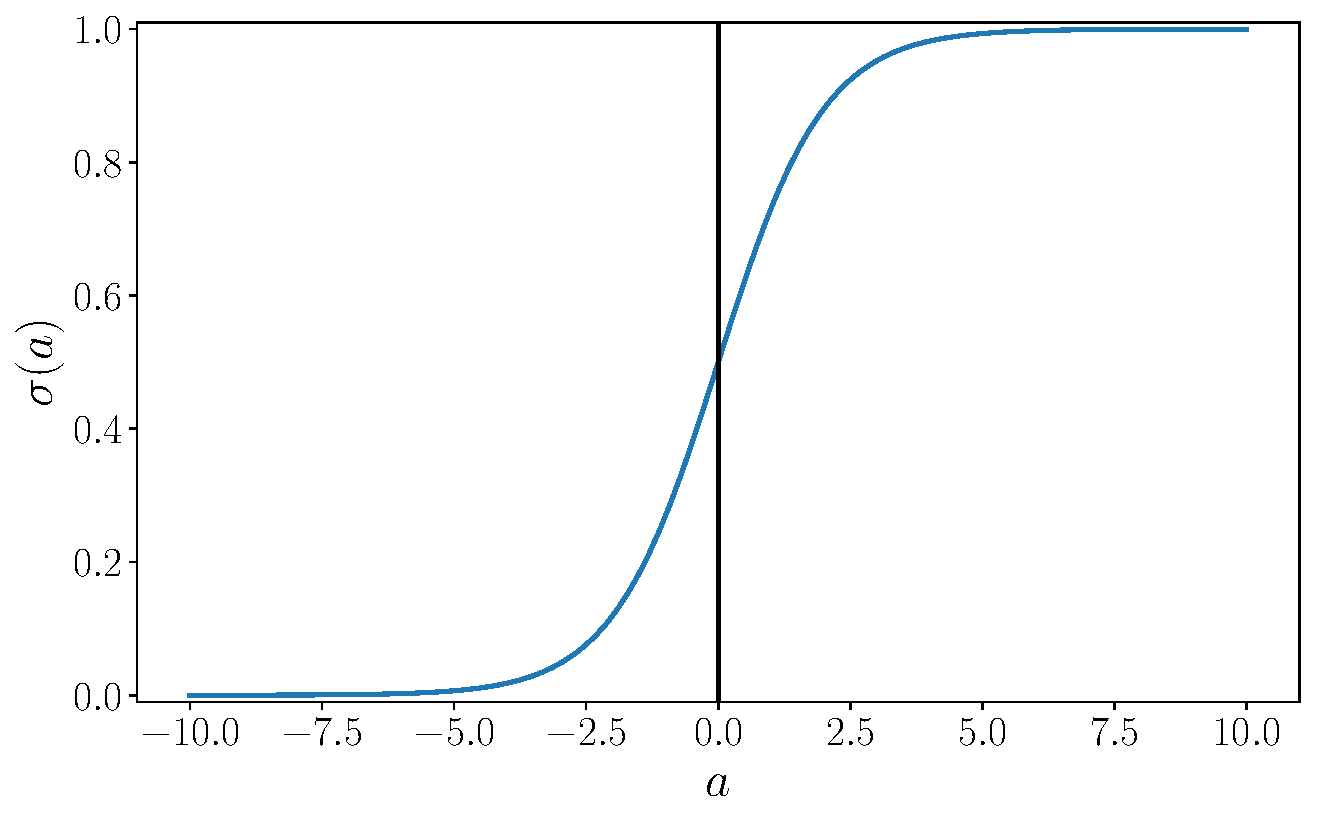
\includegraphics[height=3cm]{./figures/logistic_regression/sigmoid}
    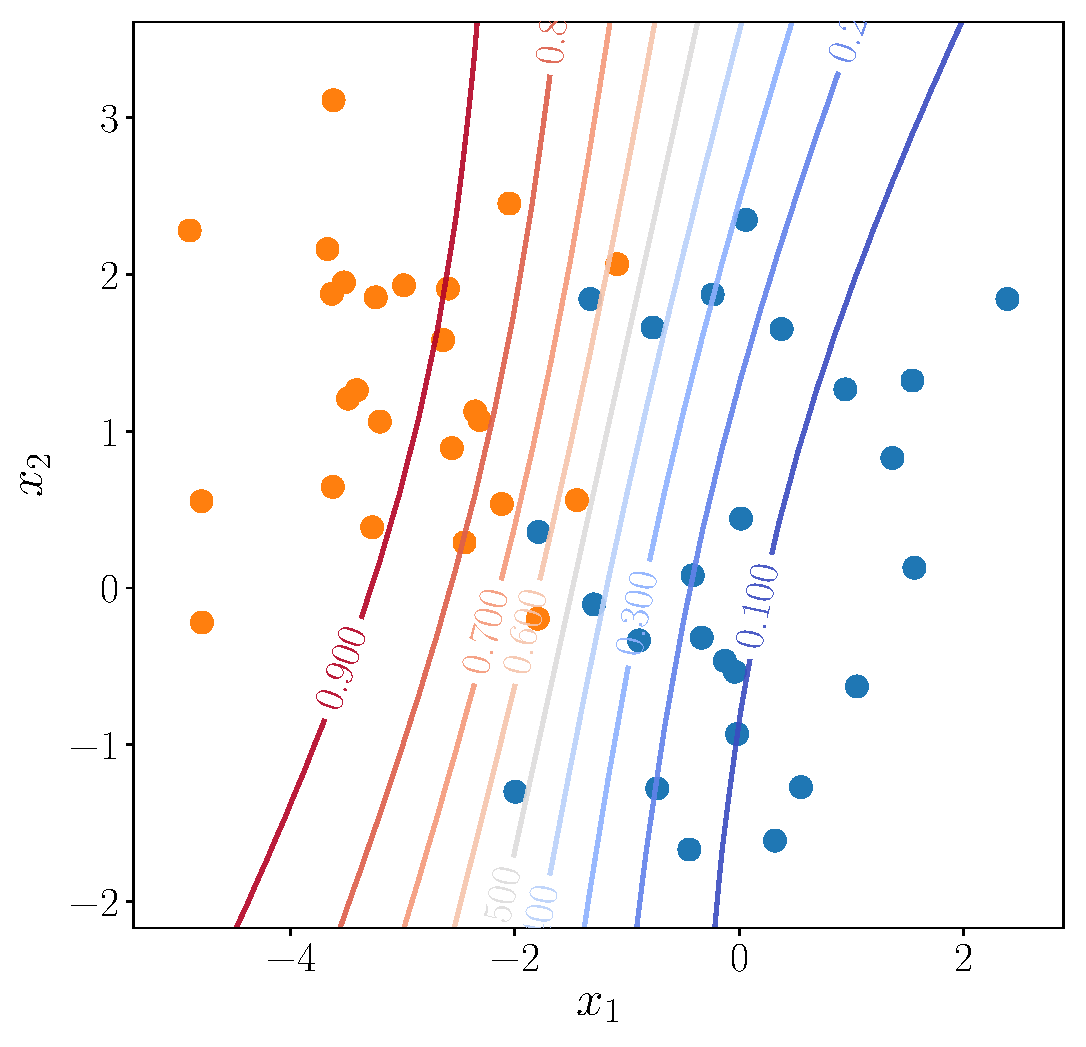
\includegraphics[height=3cm]{./figures/logistic_regression/logistic_regression_prediction}
    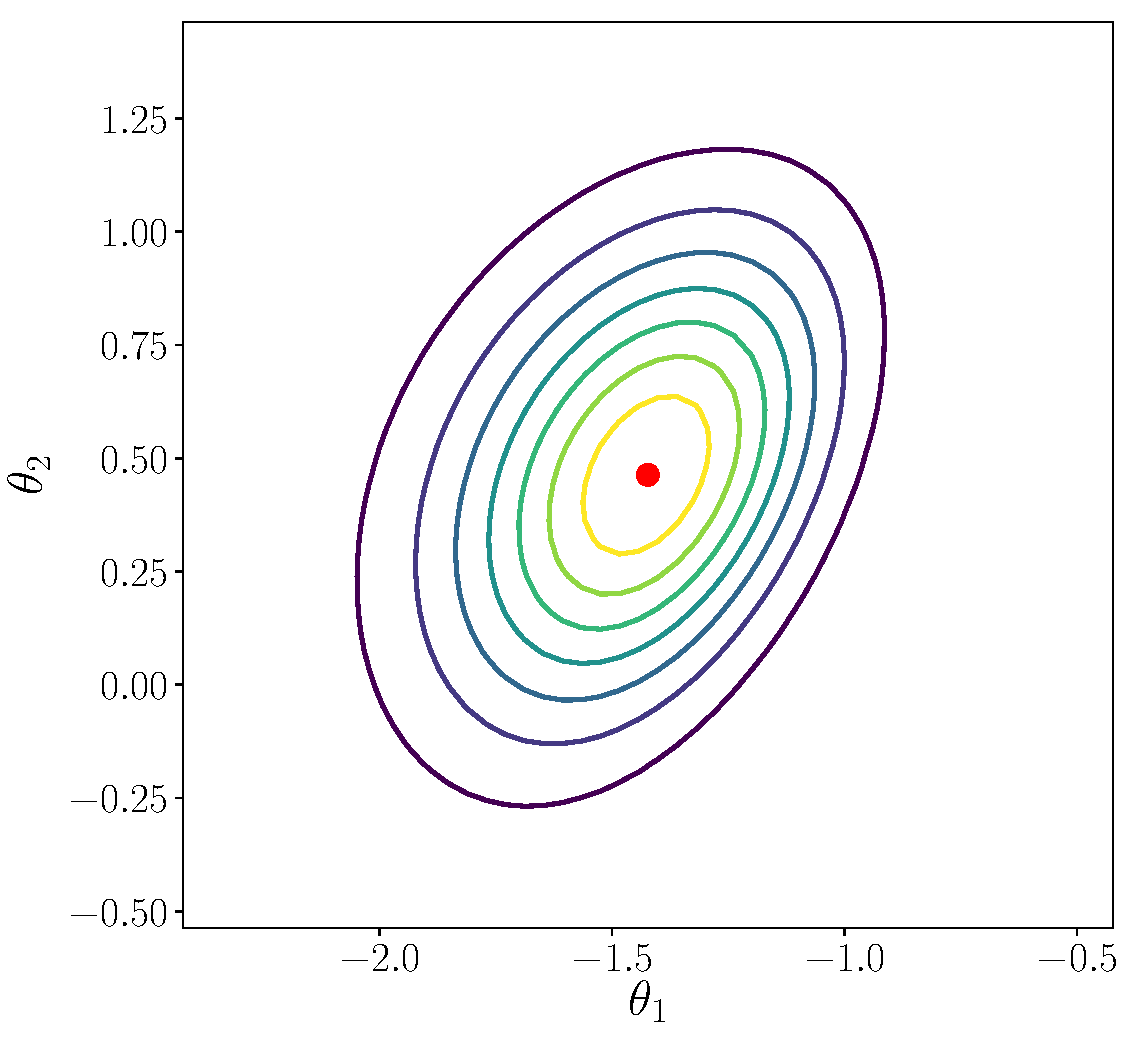
\includegraphics[height=3cm]{./figures/logistic_regression/logistic_regression_posterior}
  \end{figure}
  
  \begin{itemize}
  \item Binary classification problems
  \item Linear model with non-Gaussian likelihood
  \item Implicit modeling assumption: Gaussian $p(\vx\given\class_c)$
  \item Parameter estimation (MLE, MAP) no longer in closed form
  \item Bayesian logistic regression with Laplace approximation of the
    posterior
  \end{itemize}
\end{frame}

%%%%%%%%%%%%%%%%%%%%%%%%%%%%%%%%%%%%%%%%%
% REFERENCES
%%%%%%%%%%%%%%%%%%%%%%%%%%%%%%%%%%%%%%%%%
\begin{frame}[t,allowframebreaks]
\frametitle{References}
\linespread{1.0}
\tiny
\bibliographystyle{abbrv}
\bibliography{../includes/pi-literature}
\end{frame}



\end{document}
%%% Local Variables: 
%%% mode: latex
%%% TeX-master: t
%%% End: 
